% Options for packages loaded elsewhere
\PassOptionsToPackage{unicode}{hyperref}
\PassOptionsToPackage{hyphens}{url}
\PassOptionsToPackage{dvipsnames,svgnames,x11names}{xcolor}
%
\documentclass[
  sn-nature,
  lineno, referee]{sn-jnl}

\setlength\evensidemargin{\oddsidemargin}


\usepackage{amsmath,amssymb}
\usepackage{iftex}
\ifPDFTeX
  \usepackage[T1]{fontenc}
  \usepackage[utf8]{inputenc}
  \usepackage{textcomp} % provide euro and other symbols
\else % if luatex or xetex
  \usepackage{unicode-math}
  \defaultfontfeatures{Scale=MatchLowercase}
  \defaultfontfeatures[\rmfamily]{Ligatures=TeX,Scale=1}
\fi
\usepackage{lmodern}
\ifPDFTeX\else  
    % xetex/luatex font selection
\fi
% Use upquote if available, for straight quotes in verbatim environments
\IfFileExists{upquote.sty}{\usepackage{upquote}}{}
\IfFileExists{microtype.sty}{% use microtype if available
  \usepackage[]{microtype}
  \UseMicrotypeSet[protrusion]{basicmath} % disable protrusion for tt fonts
}{}
\makeatletter
\@ifundefined{KOMAClassName}{% if non-KOMA class
  \IfFileExists{parskip.sty}{%
    \usepackage{parskip}
  }{% else
    \setlength{\parindent}{0pt}
    \setlength{\parskip}{6pt plus 2pt minus 1pt}}
}{% if KOMA class
  \KOMAoptions{parskip=half}}
\makeatother
\usepackage{xcolor}
\setlength{\emergencystretch}{3em} % prevent overfull lines
\setcounter{secnumdepth}{-\maxdimen} % remove section numbering
% Make \paragraph and \subparagraph free-standing
\makeatletter
\ifx\paragraph\undefined\else
  \let\oldparagraph\paragraph
  \renewcommand{\paragraph}{
    \@ifstar
      \xxxParagraphStar
      \xxxParagraphNoStar
  }
  \newcommand{\xxxParagraphStar}[1]{\oldparagraph*{#1}\mbox{}}
  \newcommand{\xxxParagraphNoStar}[1]{\oldparagraph{#1}\mbox{}}
\fi
\ifx\subparagraph\undefined\else
  \let\oldsubparagraph\subparagraph
  \renewcommand{\subparagraph}{
    \@ifstar
      \xxxSubParagraphStar
      \xxxSubParagraphNoStar
  }
  \newcommand{\xxxSubParagraphStar}[1]{\oldsubparagraph*{#1}\mbox{}}
  \newcommand{\xxxSubParagraphNoStar}[1]{\oldsubparagraph{#1}\mbox{}}
\fi
\makeatother


\providecommand{\tightlist}{%
  \setlength{\itemsep}{0pt}\setlength{\parskip}{0pt}}\usepackage{longtable,booktabs,array}
\usepackage{calc} % for calculating minipage widths
% Correct order of tables after \paragraph or \subparagraph
\usepackage{etoolbox}
\makeatletter
\patchcmd\longtable{\par}{\if@noskipsec\mbox{}\fi\par}{}{}
\makeatother
% Allow footnotes in longtable head/foot
\IfFileExists{footnotehyper.sty}{\usepackage{footnotehyper}}{\usepackage{footnote}}
\makesavenoteenv{longtable}
\usepackage{graphicx}
\makeatletter
\newsavebox\pandoc@box
\newcommand*\pandocbounded[1]{% scales image to fit in text height/width
  \sbox\pandoc@box{#1}%
  \Gscale@div\@tempa{\textheight}{\dimexpr\ht\pandoc@box+\dp\pandoc@box\relax}%
  \Gscale@div\@tempb{\linewidth}{\wd\pandoc@box}%
  \ifdim\@tempb\p@<\@tempa\p@\let\@tempa\@tempb\fi% select the smaller of both
  \ifdim\@tempa\p@<\p@\scalebox{\@tempa}{\usebox\pandoc@box}%
  \else\usebox{\pandoc@box}%
  \fi%
}
% Set default figure placement to htbp
\def\fps@figure{htbp}
\makeatother

%%%% Standard Packages

\usepackage{graphicx}%
\usepackage{multirow}%
\usepackage{amsmath,amssymb,amsfonts}%
\usepackage{amsthm}%
\usepackage{mathrsfs}%
\usepackage[title]{appendix}%
\usepackage{xcolor}%
\usepackage{textcomp}%
\usepackage{manyfoot}%
\usepackage{booktabs}%
\usepackage{algorithm}%
\usepackage{algorithmicx}%
\usepackage{algpseudocode}%
\usepackage{listings}%
\usepackage[euler]{textgreek}%

%%%%

\raggedbottom
\makeatletter
\@ifpackageloaded{float}{}{\usepackage{float}}
\floatstyle{plain}
\@ifundefined{c@chapter}{\newfloat{supplemental}{h}{losup}}{\newfloat{supplemental}{h}{losup}[chapter]}
\floatname{supplemental}{Supplementary Material}
\newcommand*\listofsupplementals{\listof{supplemental}{List of Supplementary Materials}}
\makeatother
\makeatletter
\@ifpackageloaded{caption}{}{\usepackage{caption}}
\AtBeginDocument{%
\ifdefined\contentsname
  \renewcommand*\contentsname{Table of contents}
\else
  \newcommand\contentsname{Table of contents}
\fi
\ifdefined\listfigurename
  \renewcommand*\listfigurename{List of Figures}
\else
  \newcommand\listfigurename{List of Figures}
\fi
\ifdefined\listtablename
  \renewcommand*\listtablename{List of Tables}
\else
  \newcommand\listtablename{List of Tables}
\fi
\ifdefined\figurename
  \renewcommand*\figurename{Figure}
\else
  \newcommand\figurename{Figure}
\fi
\ifdefined\tablename
  \renewcommand*\tablename{Table}
\else
  \newcommand\tablename{Table}
\fi
}
\@ifpackageloaded{float}{}{\usepackage{float}}
\floatstyle{ruled}
\@ifundefined{c@chapter}{\newfloat{codelisting}{h}{lop}}{\newfloat{codelisting}{h}{lop}[chapter]}
\floatname{codelisting}{Listing}
\newcommand*\listoflistings{\listof{codelisting}{List of Listings}}
\makeatother
\makeatletter
\makeatother
\makeatletter
\@ifpackageloaded{caption}{}{\usepackage{caption}}
\@ifpackageloaded{subcaption}{}{\usepackage{subcaption}}
\makeatother

\usepackage{bookmark}

\IfFileExists{xurl.sty}{\usepackage{xurl}}{} % add URL line breaks if available
\urlstyle{same} % disable monospaced font for URLs
\hypersetup{
  pdftitle={Soil Microbial Functional Succession Over One Year of Human Decomposition},
  pdfauthor={Allison R. Mason; Lois S. Taylor; Naomi E. Gilbert; Steven W. Wilhelm; Jennifer M. DeBruyn},
  pdfkeywords={Human Decomposition, Microbial
Succession, Metatranscriptomics, Soil Microbial Ecology},
  colorlinks=true,
  linkcolor={blue},
  filecolor={Maroon},
  citecolor={Blue},
  urlcolor={Blue},
  pdfcreator={LaTeX via pandoc}}


\title[Soil Microbial Functional Succession Over One Year of Human
Decomposition]{Soil Microbial Functional Succession Over One Year of
Human Decomposition}

% author setup
\author[1]{\fnm{Allison R.} \sur{Mason}}\author[2]{\fnm{Lois S.} \sur{Taylor}}\author[1]{\fnm{Naomi E.} \sur{Gilbert}}\author[1]{\fnm{Steven W.} \sur{Wilhelm}}\author*[1,2]{\fnm{Jennifer M.} \sur{DeBruyn}}\email{jdebruyn@utk.edu}
% affil setup
\affil[1]{\orgdiv{Department of Microbiology}, \orgname{University of
Tennessee-Knoxville}, \orgaddress{\street{1311 Cumberland
Avenue}, \city{Knoxville}, \postcode{37996}}}
\affil[2]{\orgdiv{Department of Biosystems Engineering and Soil
Science}, \orgname{University of
Tennessee-Knoxville}, \orgaddress{\street{2506 E.J. Chapman
Drive}, \city{Knoxville}, \postcode{37996}}}

% abstract 

\abstract{During terrestrial vertebrate decomposition, host and
environmental microbial communities work together to drive
biogeochemical cycling of carbon and nutrients. These mixed communities
undergo dramatic restructuring in the resulting decomposition hotspots.
To reveal the succession of both the active microbial members and the
metabolic pathways they use, we generated metatranscriptomes from soil
samples collected over one year from below three decomposing human
bodies. Soil microbes increased expression of ``heat shock'' proteins in
response to decomposition products changing physiochemical conditions
(\emph{i.e.}, reduced oxygen, high salt). Increased fungal lipase
expression implicated fungi as key decomposers of fat tissue. Expression
of nitrogen cycling genes was phased with soil oxygen concentrations:
during hypoxic soil conditions, genes catalyzing N-reducing processes
(\emph{e.g.}, hydroxylamine to nitric oxide and nitrous oxide to
nitrogen gas during reduced oxygen conditions) were increased, followed
by increased expression of nitrification genes once oxygen diffused back
into the soil. Increased expression of bile salt hydrolases implicated a
microbial source for the high concentrations of taurine typically
observed during vertebrate decomposition. Collectively, microbial gene
expression profiles remained altered even after one year. Together, we
show how human decomposition alters soil microbial gene expression,
revealing both ephemeral and lasting effects on soil microbial
communities.}

% keywords
\keywords{Human Decomposition,  Microbial
Succession,  Metatranscriptomics,  Soil Microbial Ecology}

\begin{document}
\maketitle


\section{Introduction}\label{introduction}

Soil microbial communities are important drivers of ecosystem processes
in terrestrial environments. Many soil microbes are decomposers that
degrade complex organic matter and drive nutrient cycling in terrestrial
ecosystems. Environmental disturbances can impact the presence and/or
activity of soil microorganisms involved in these cycles, ultimately
affecting nutrient availability and greenhouse gas emissions, such as
CO\textsubscript{2} and N\textsubscript{2}O
\citep{benninger_biochemical_2008, towne_prairie_2000}. Vertebrate death
and subsequent carcass deposition in terrestrial ecosystems is one
disturbance resulting in the deposition of large quantities of organic C
and N
\citep{debruyn_carrion_2024, parmenter_carrion_2009, macdonald_carrion_2014, bump_ungulate_2009, aitkenhead-peterson_mapping_2012, keenan_mortality_2018, fancher_evaluation_2017, quaggiotto_dynamic_2019},
along with other elements (P, K, S, \emph{etc})
\citep{taylor_soil_2023}, which collectively contribute to
microbially-mediated biogeochemical cycling. In addition to this,
changes in pH, temperature, and fluctuations in soil oxygen provide
abiotic filtering further impacting microbial metabolic strategies
\citep{aitkenhead-peterson_mapping_2012, keenan_mortality_2018, fancher_evaluation_2017, taylor_soil_2023, mason_body_2022, taylor_transient_2024}.
Vertebrate decomposition also results in mixing of host and
environmental microbes: the animal's microflora are flushed into the
soil along with decomposition products where they further contribute to
decomposition processes (\emph{e.g.}, organic nitrogen mineralization)
\citep{keenan_microbial_2023}.

While C and N transformations have been documented during decomposition,
the functional response of microbes and their roles in nutrient cycles
remain unclear. The composition and structure of decomposition-impacted
soil microbial communities have been investigated using sequencing of
marker genes amplicons (\emph{i.e.}, 16S rRNA, 18S rRNA, ITS). This has
allowed for the identification of changes in microbial biodiversity and
taxonomic succession in response to vertebrate decomposition, revealing
patterns that include increases in the anaerobic taxa \emph{Firmicutes}
and \emph{Bacteroidetes} \citep{mason_microbial_2023}. However, few
studies have integrated soil biogeochemistry with microbial community
composition, which can further help to describe microbial ecology in
these decomposition systems. Taylor et al.~(2024)
\citep{taylor_transient_2024} showed that fungal community shifts were
linked to changes in soil dissolved oxygen, highlighting interactions
between soil microbes and changes in the surrounding environment. While
insightful for making potential connections between taxa and
environment, these analyses do not inform which taxa are active members
of the community, which functional pathways/genes are expressed, and how
these pathways facilitate decomposition processes.

RNA sequencing (\emph{i.e.}, metatranscriptomics) and metabolomics can
be used to investigate microbial community functional succession during
decomposition. They can identigy how ecological functions, including C
and N cycling, are impacted by decomposition events in terrestrial
ecosystems. To date, applications of metatranscriptomics to vertebrate
decomposition samples have been limited to internal host communities
\citep{burcham_total_2019, ashe_characterization_2021}: Burcham et
al.~(2019) \citep{burcham_total_2019} revealed differential expression
of amino acid and carbohydrate metabolism in the heart during mouse
decomposition, while Ashe et al.~(2021)
\citep{ashe_characterization_2021} documented taxonomic shifts in gene
expression of oral microbial communities during human decomposition.

We expected that the impacted soil microbial community, which includes a
mix of host and environmental taxa, would also have altered gene
expression profiles, given the release of decomposition byproducts into
the soil during terrestrial decomposition. We previously assessed the
decomposition-impacted soil metabolome \citep{debruyn_comparative_2021},
demostrating a prevalence of amino acids and suggesting upregulation of
organic nitrogen metabolic pathways. Additionally, DeBruyn et al.~(2021)
\citep{debruyn_comparative_2021} showed the soil metabolome was
surprisingly still altered compared to starting conditions at the end of
that 21-week study, suggesting long-term impacts of decomposition on
soil microbial functioning.

Here, we investigated soil microbial gene expression during a one-year
period of human decomposition. The overarching goal of this work was to
assess the effects of vertebrate decomposition on ecosystem function by
characterizing community-level shifts in soil microbial function. We
hypothesized that: (i) gene expression would shift over time as
resources were consumed and transformed and soil chemical and physical
conditions changed due to the influx of decomposition products during
soft tissue degradation
\citep{keenan_mortality_2018, fancher_evaluation_2017, debruyn_comparative_2021};
(ii) gene expression for enzymes involved in nitrogen cycling would be
altered, as changes in nitrogen pools have been previously described in
decomposition soils \citep{keenan_mortality_2018}; (iii) expression of
genes involved in lipid metabolism would increase, as lipids from the
body entered the soil during decomposition and previous studies
identified lipolytic organisms in decomposition soils
\citep{howard_characterization_2010, mason_body_2022}; (iv) microbial
expression profiles in the impacted soil would remain altered even after
a year, as previous studies have shown that community composition
\citep{cobaugh_functional_2015, singh_temporal_2018} can remain altered
longer than a year. We analyzed metatranscriptomes of soil samples
collected at six key timepoints over one year of human decomposition to
determine the identity of active populations and the expression of genes
and pathways relevant to the enhanced biogeochemical cycling observed in
decomposition hotspots. We compared gene expression between
decomposition timepoints and control soils that were unexposed to
decomposition products to identify functions or functional pathways of
interest. We show: (i) decomposition shifts soil microbial community
gene expression, with the effects still measurable after one year; (ii)
expression of genes related to stress response are elevated in
decomposition soils; (iii) expression of genes encoding triacylglycerol
lipase differed between fungi (increased) and bacteria (decreased); (iv)
evidence for phased nitrification and denitrification, driven by changes
in soil dissolved oxygen; (v) evidence for organic sulfur processing
(taurine) via bile salt hydrolases. This direct assessment of function
expands the fudamental understanding of terrestrial vertebrate
decomposition, providing insight into pathways of biogeochemical cycling
within these hotsopts.

\section{Results}\label{results}

\subsection{Soil Physiochemistry}\label{soil-physiochemistry}

Soil chemistry was altered in response to the presence of a decomposing
human cadaver, with multiple parameters still impacted after one year
\citep{taylor_transient_2024}. Generally, soil pH decreased and remained
low in decomposition soils of all but one individual. Soil electrical
conductivity (EC) increased in response to decomposition, remaining
elevated through approximately day 58 before gradually decreasing
throughout the remainder of the study
(Supplementary Material~\ref{sup-chem-plot}). Respiration (evolved
CO\textsubscript{2}) increased by an order of magnitude beginning at day
12, which corresponded to a reduction in soil dissolved oxygen (DO) to
29\% - 48.9\%. Ammonium concentrations increased 78-fold, reaching
maximum concentrations between days 12 and 58. This was followed by
decreased ammonium and increased nitrate concentrations at day 86, with
nitrate concentrations reaching a maximum at day 168
(Supplementary Material~\ref{sup-chem-plot}).

\subsection{Microbial gene expression in response to human
decomposition}\label{microbial-gene-expression-in-response-to-human-decomposition}

Gene expression profiles in decomposition-impacted soils shifted away
from controls and day zero samples as decomposition progressed
(Fig~\ref{fig-mds}A). Expression was most different from controls on
study days 58, 86, 168 (Supplementary Material~\ref{sup-heatmap-plot}),
before returning toward control conditions on study day 376. After one
year of decomposition, soil gene expression profiles had not returned to
pre-decomposition conditions, as evidenced by their clustering away from
controls and day zero samples in the MDS plot (Fig~\ref{fig-mds}A).

% Place figure captions after the first paragraph in which they are cited.
\begin{figure}[!h]
\caption{{\bf Microbial gene expression profiles are altered during human decomposition.}
Multidimensional scaling (MDS) shows gene expression within soils changed as decomposition progressed (A). Additionally, canonical correspondence analysis (CCA) shows that environmental variables explained 47.3\% of the variation in gene expression profiles (B). Variables in bold red type significantly (p < 0.05) explained some of the variation in gene expression profiles as assessed by Permutational Analysis of Variance (PERMANOVA). In both panels soils from controls (CON) and the three donors (SP1, SP2, SP3) are denoted by symbol shape, while color represents study day. In B, soil physiochemical variable loadings are represented by arrows: Gravimetric water content (GWC), electrical conductivity (EC), pH (pH), dissolved oxygen (DO), respiration (evolved CO\textsubscript{2}\ \textmu mol gdw\textsuperscript{-1}), ammonium (NH\textsubscript{4}), and nitrate (NO\textsubscript{3}) concentrations (mg gdw\textsuperscript{-1}), percent carbon (\%C), percent nitrogen (\%N), carbon:nitrogen ratio (C:N), ambient temperature (T\textsubscript{A}), and soil temperature (T\textsubscript{S}).}
\label{fig-mds}
\end{figure}

\pandocbounded{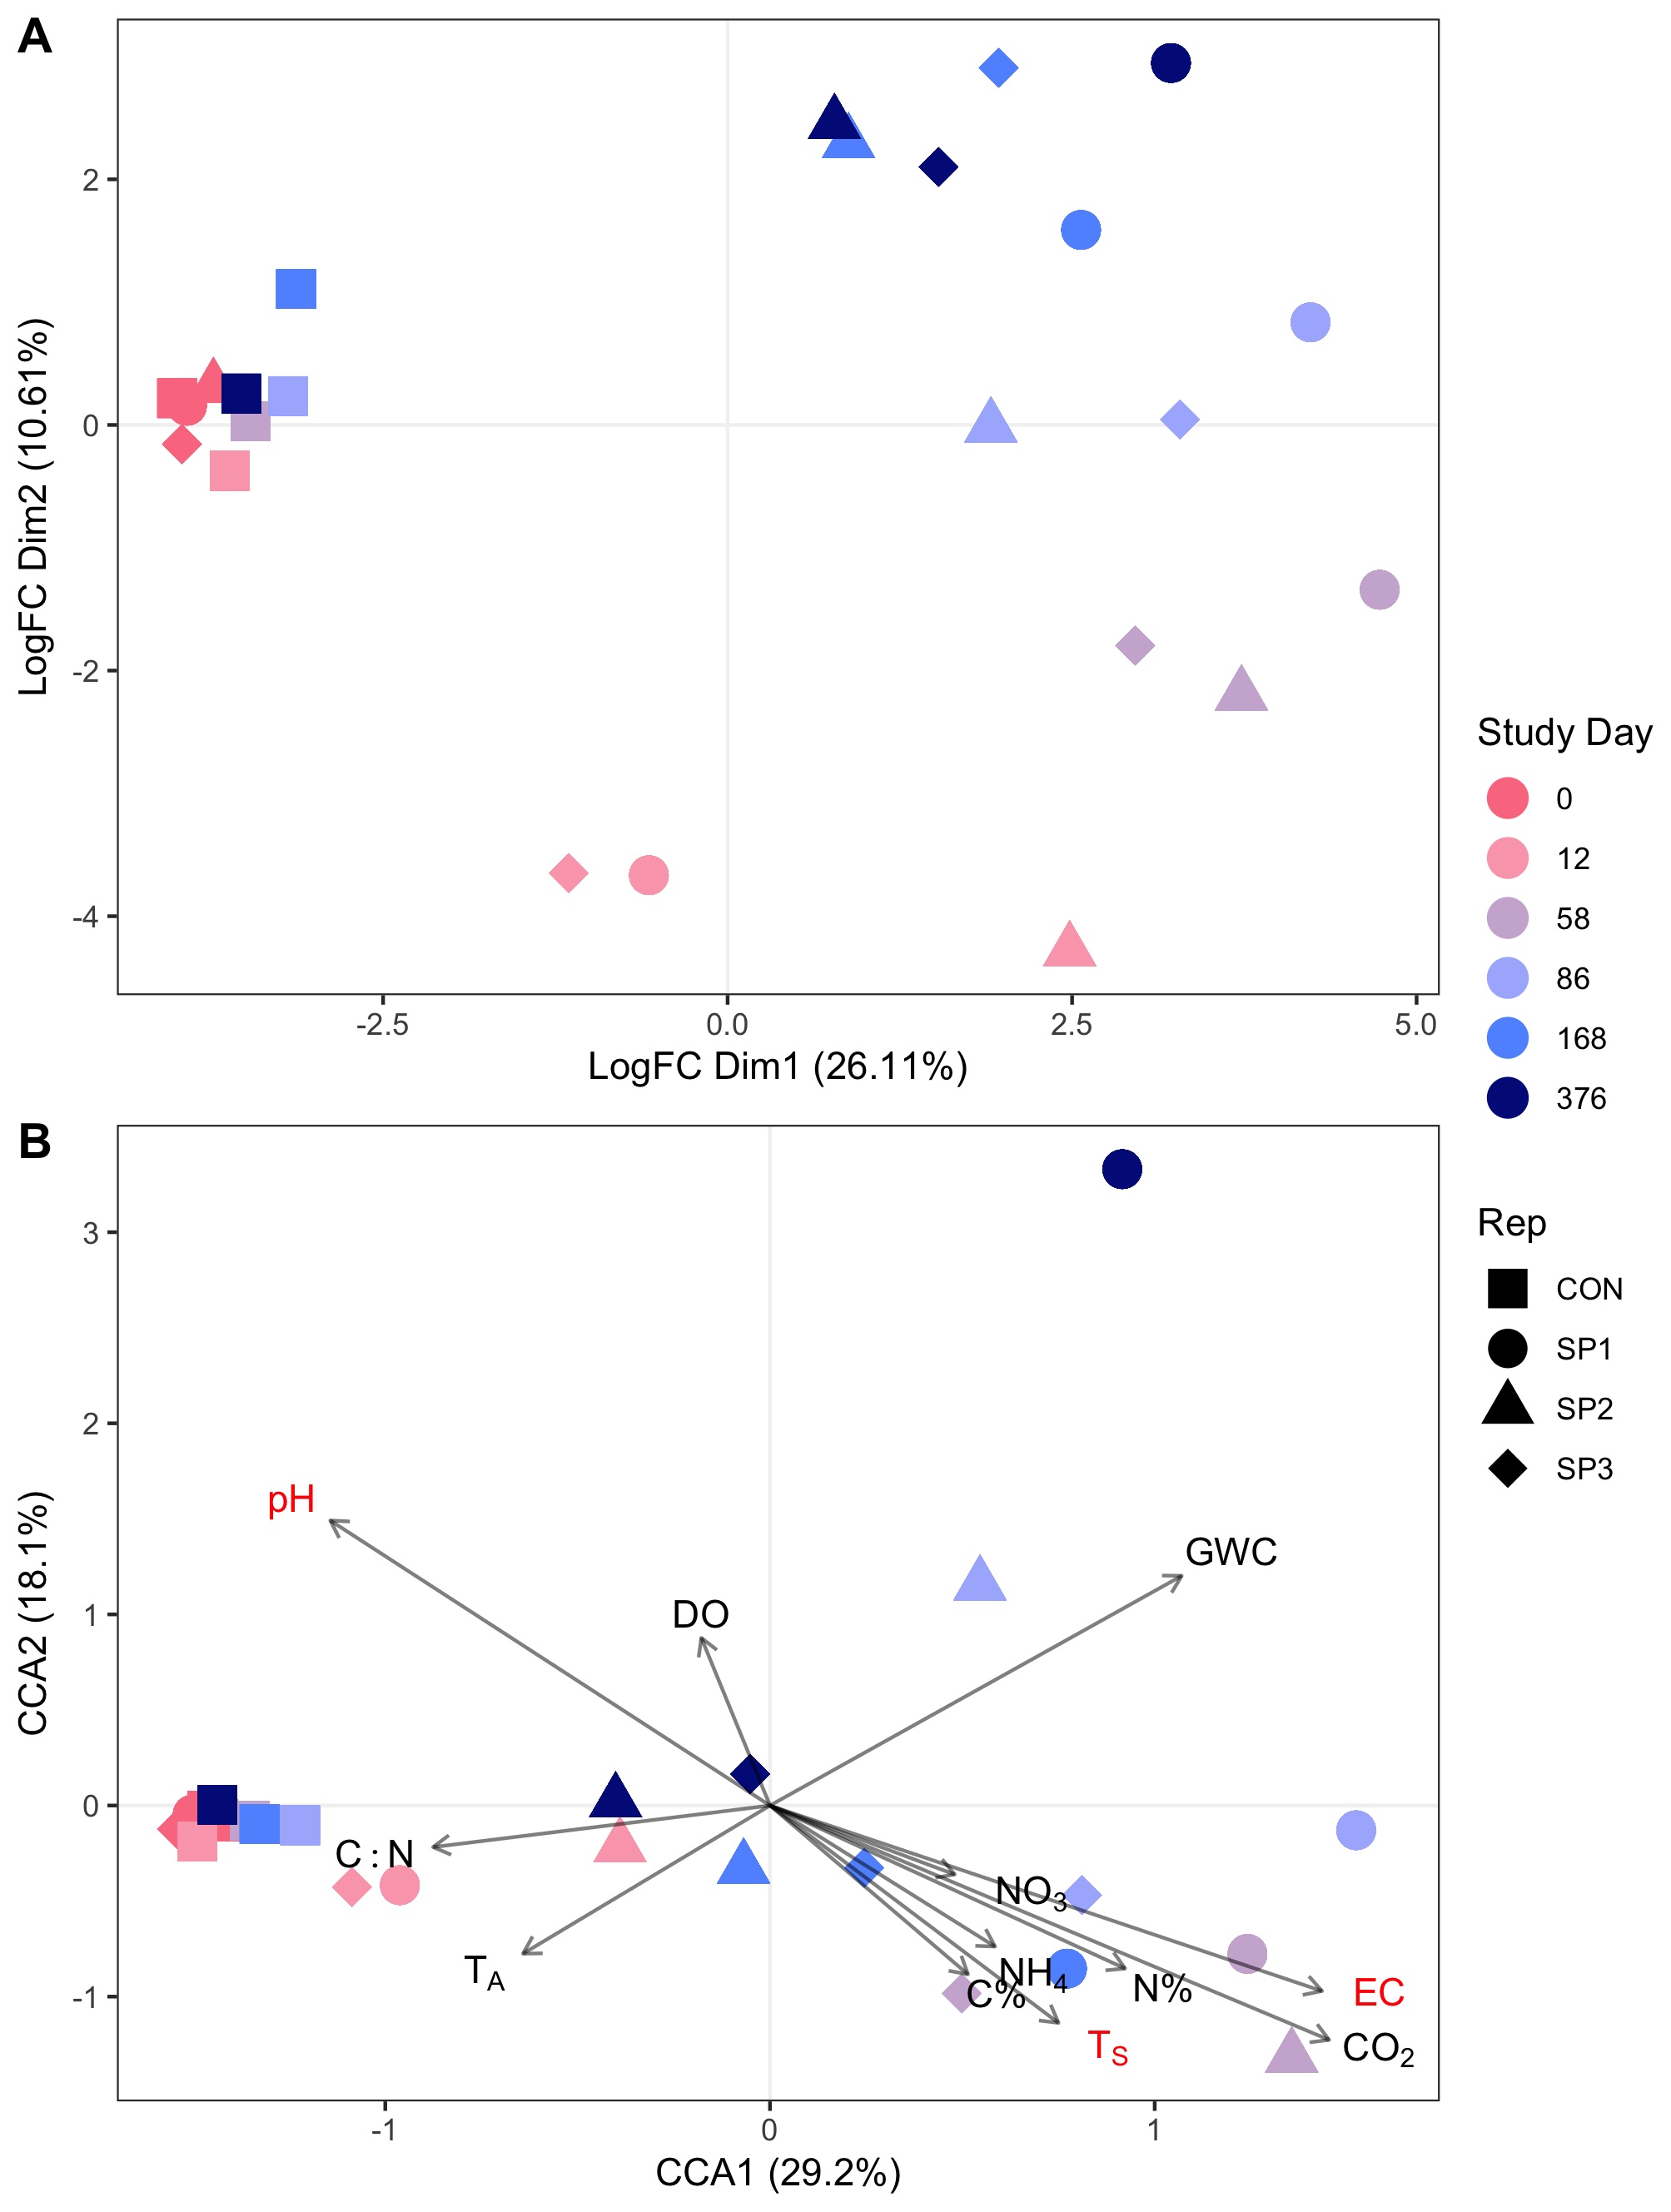
\includegraphics[keepaspectratio]{../../figures/Fig1.png}}

Some correlations were observed between gene expression shifts and soil
physiochemical data at decomposition timepoints. Canonical
correspondence analysis (CCA) was used to constrain gene expression data
with soil physiochemical data (Fig~\ref{fig-mds}B). CCA1 and CCA2
explained 29.2\% and 18.1\% of the variance in gene expression,
respectively. Transcript profiles at day 12 were associated with an
increase in soil carbon to nitrogen ratio (C:N). Gene expression
profiles at days 58 to 86 were positively correlated with increased soil
temperature, EC, and evolved CO\textsubscript{2}, while study day 168
was associated with elevated levels of soil NO\textsubscript{3}.
Further, Permutational Analysis of Variance (PERMANOVA) revealed that
internal accumulated degree hours (ADH), soil temperature, pH, and EC
significantly explained some of the variation in gene expression
profiles (p \textless{} 0.05). No other soil chemical variables were
significant at \textalpha~= 0.05
(Supplementary Material~\ref{sup-tbl-cca-panova}).

Overall, decomposition changed soil gene expression profiles over the
one-year study relative to control soils. Differential expression
analysis between decomposition and control soils identified 7,047
down-regulated and 38,425 up-regulated genes. Gene transcripts that were
associated with control soils belonged to a wide variety of clusters of
orthologous genes (COG) functional categories. Specifically, the top 20
genes whose expression was higher in control soils belonged to ten
unique COG categories, including signal transduction mechanisms,
transcription, and those of unknown function. In contrast, the top 20
genes whose expression was higher in decomposition soils only fell into
four COG categories (Supplementary Material~\ref{sup-t30-trt-plot} A):
1) post-translational modification, protein turnover, and chaperones; 2)
energy production and conversion; 3) cell motility; and 4) carbohydrate
transport and metabolism. The most common COG category represented in
decomposition soils (80\% of the top 20 genes) was post-translational
modification, protein turnover, and chaperones. Within this category,
several heat shock stress response genes were identified, including
SSA2, HSP82, and clpB (Supplementary Material~\ref{sup-t30-trt-tbl}).
Further investigation of these genes over time shows that their
expression increased, typically reaching maximum transcript levels
around study days 58 and 86 (Fig~\ref{fig-heatshock}). This corresponded
to elevated soil temperatures below decomposing bodies between study
days 12-80, with soil temperatures increasing to approximately 43°C
\citep{taylor_transient_2024}, as well as maximum soil EC and minimum
dissolved oxygen measurements between days 12 and 58
(Supplementary Material~\ref{sup-chem-plot}).

% Place figure captions after the first paragraph in which they are cited.
\begin{figure}[!h]
\caption{{\bf Normalized log2 expression of heat shock proteins identified by differential expression analysis comparing decomposition and control soils.}
Each panel represents a single heat shock transcript, labeled with query ID. Symbol color denotes if the sample is a control (CON, green), or one of three individuals: SP1 (orange), SP2 (purple), or SP3 (pink).}
\label{fig-heatshock}
\end{figure}

\pandocbounded{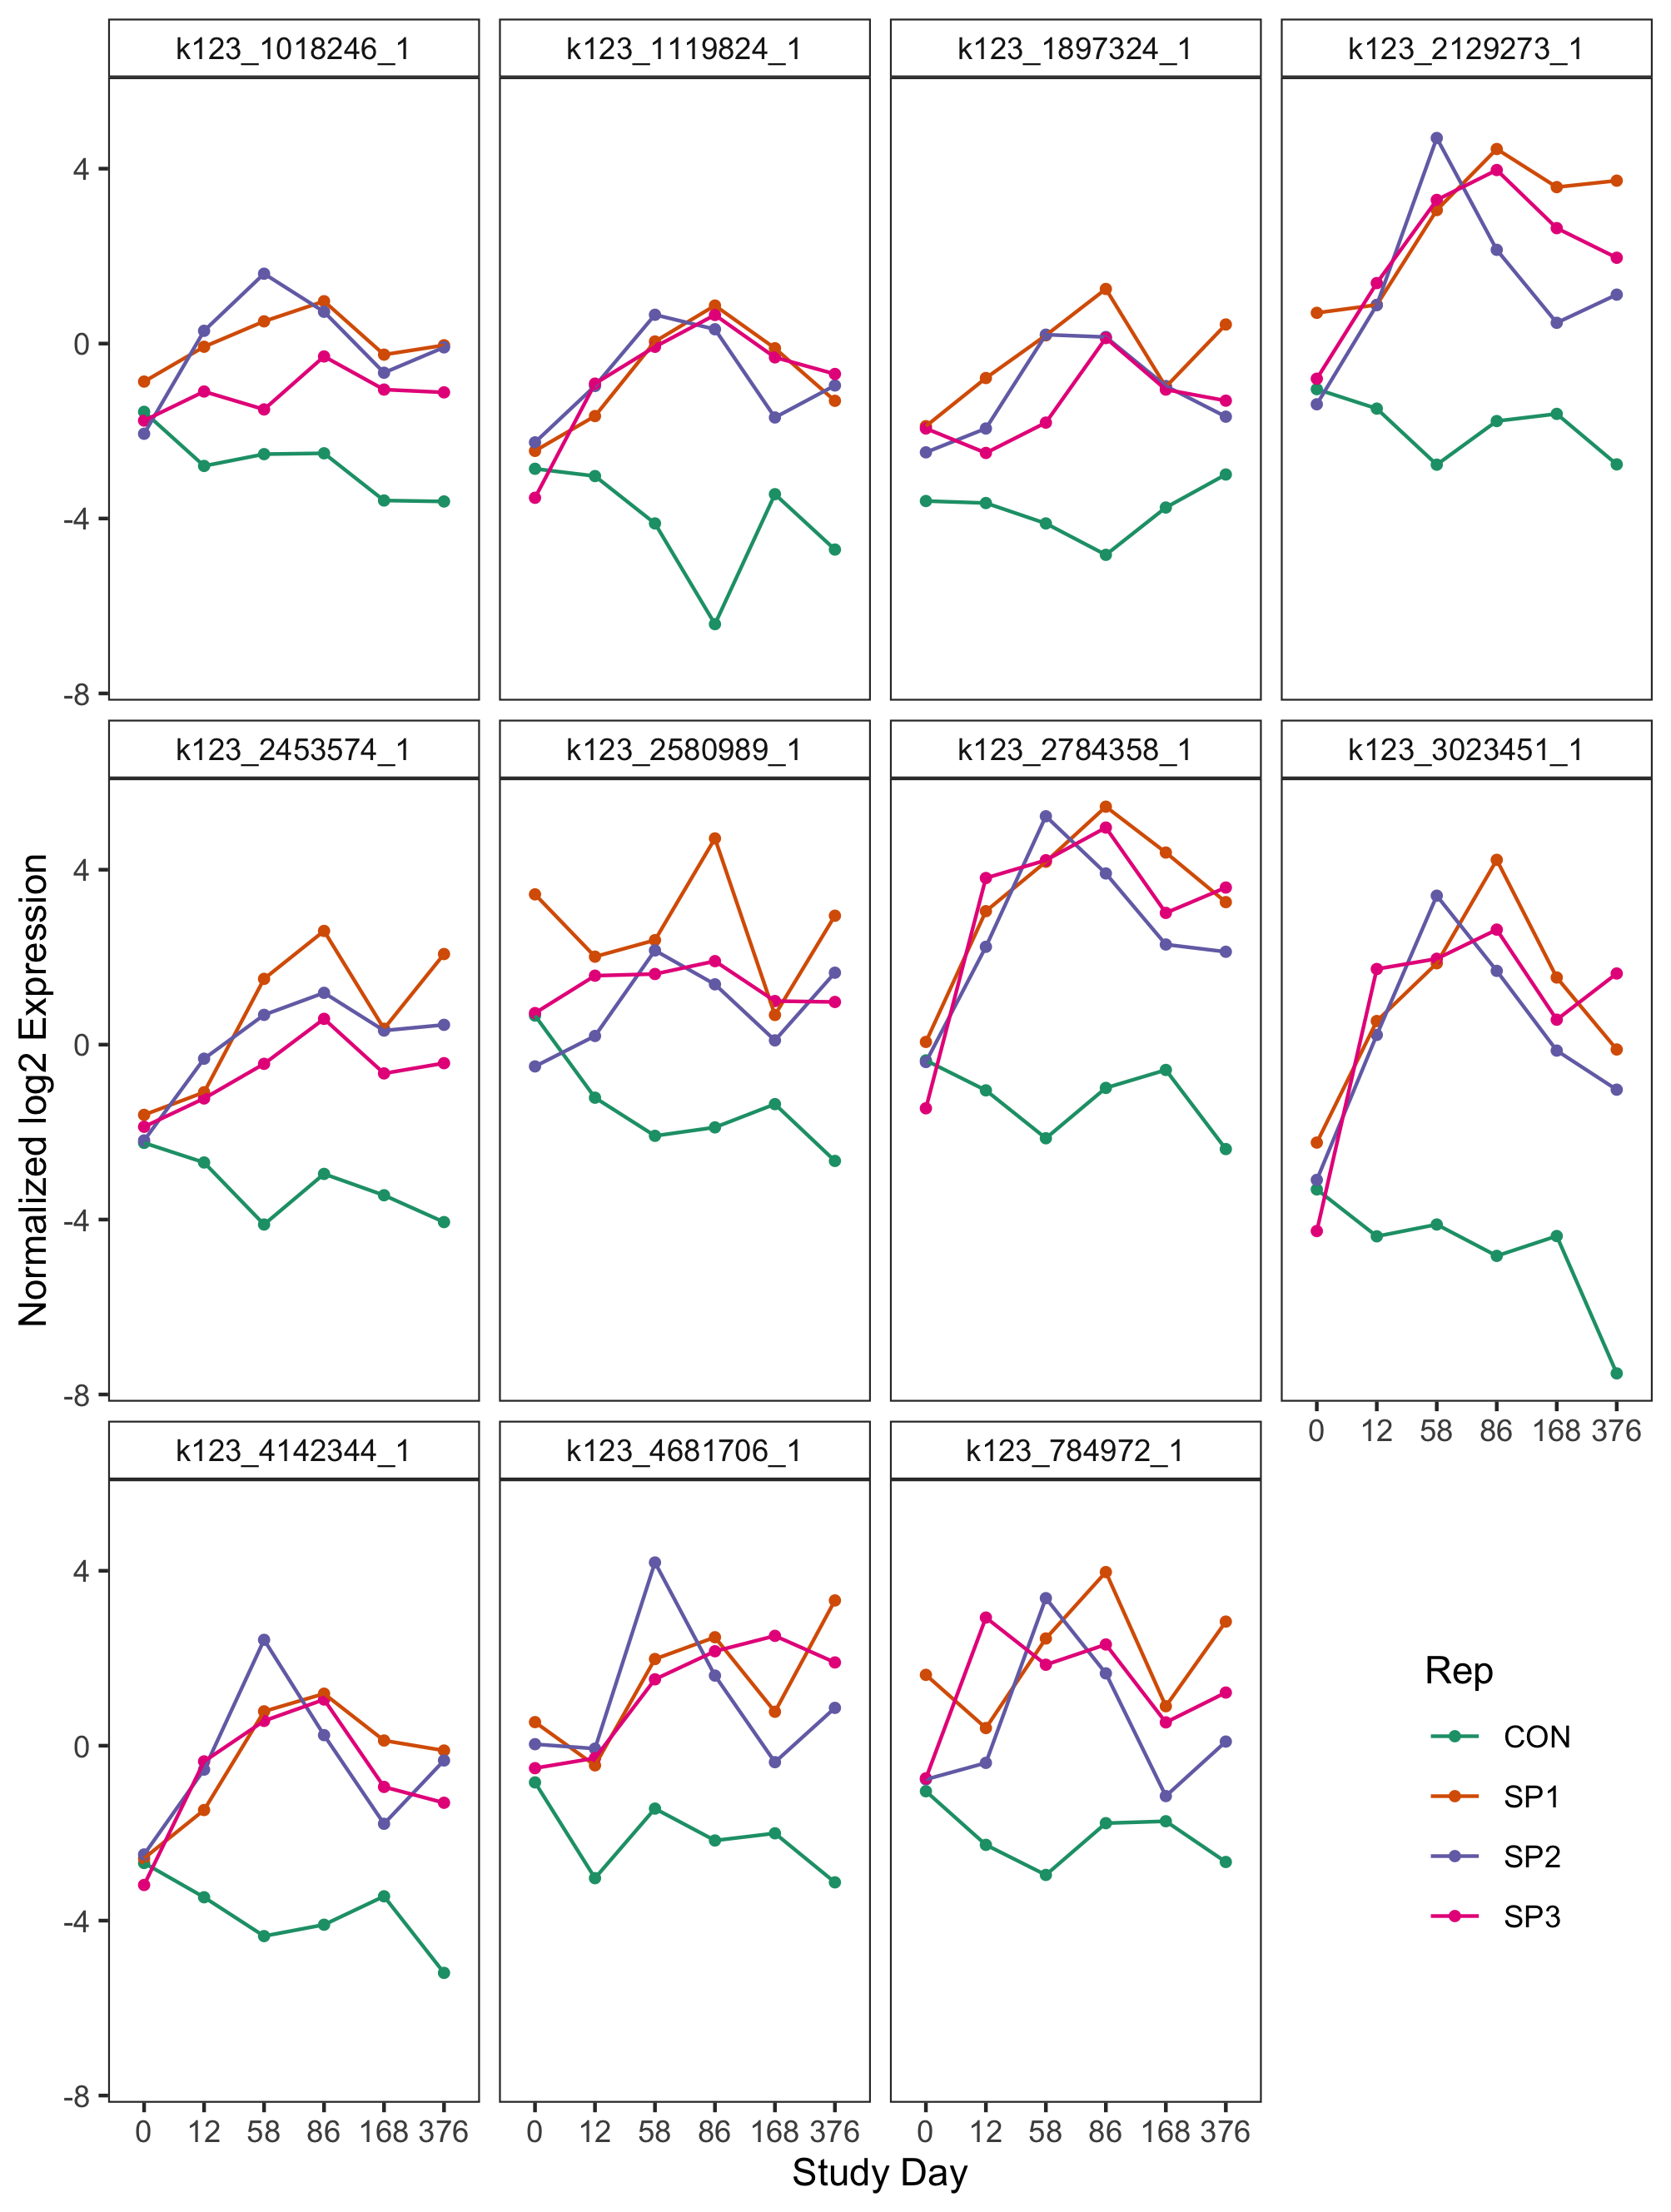
\includegraphics[keepaspectratio]{../../figures/Trt_DE_top15_heatshockTPM.png}}

Taxonomy associated with top differentially expressed gene transcripts
also differed between control and decomposition soils. The top 40
significantly differentially expressed gene transcripts in decomposition
soils were associated with Fungi, \emph{Actinobacteria}, and
\emph{Xanthomonadales}, while gene transcripts in controls were
associated with \emph{Acidobacteria}, \emph{Cyanobacteria},
\emph{Proteobacteria} (\textalpha, \textdelta, \textgamma), and
\emph{Planctomycetes} (Supplementary Material~\ref{sup-t30-trt-plot} B).
The greatest number of differentially expressed genes relative to
control samples was observed at day 86, where we saw 145,460 and 124,883
up- and down-regulated genes, respectively.

\subsection{Temporal gene expression shows shifted in decomposer
functions}\label{temporal-gene-expression-shows-shifted-in-decomposer-functions}

Differential expression analysis between sequential study days revealed
which genes were altered during decomposition time. The top ten
significantly up- and down-regulated genes, determined by the lowest
p-values from differential expression analysis (cutoff =
\textalpha~\textless{} 0.05), are reported in
Supplementary Material~\ref{sup-t20-day-tbl} and
Fig~\ref{fig-top-day-bar}.

% Place figure captions after the first paragraph in which they are cited.
\begin{figure}[!h]
\caption{{\bf Top twenty up- and down-regulated genes in decomposition soils comparing sequential study days (0, 12, 58, 86, 168, 376) colored by COG functional category (A) and taxonomic annotation (B).}
Positive values denote increased expression compared to the preceding timepoint, while negative values denote a decrease.}
\label{fig-top-day-bar}
\end{figure}

\pandocbounded{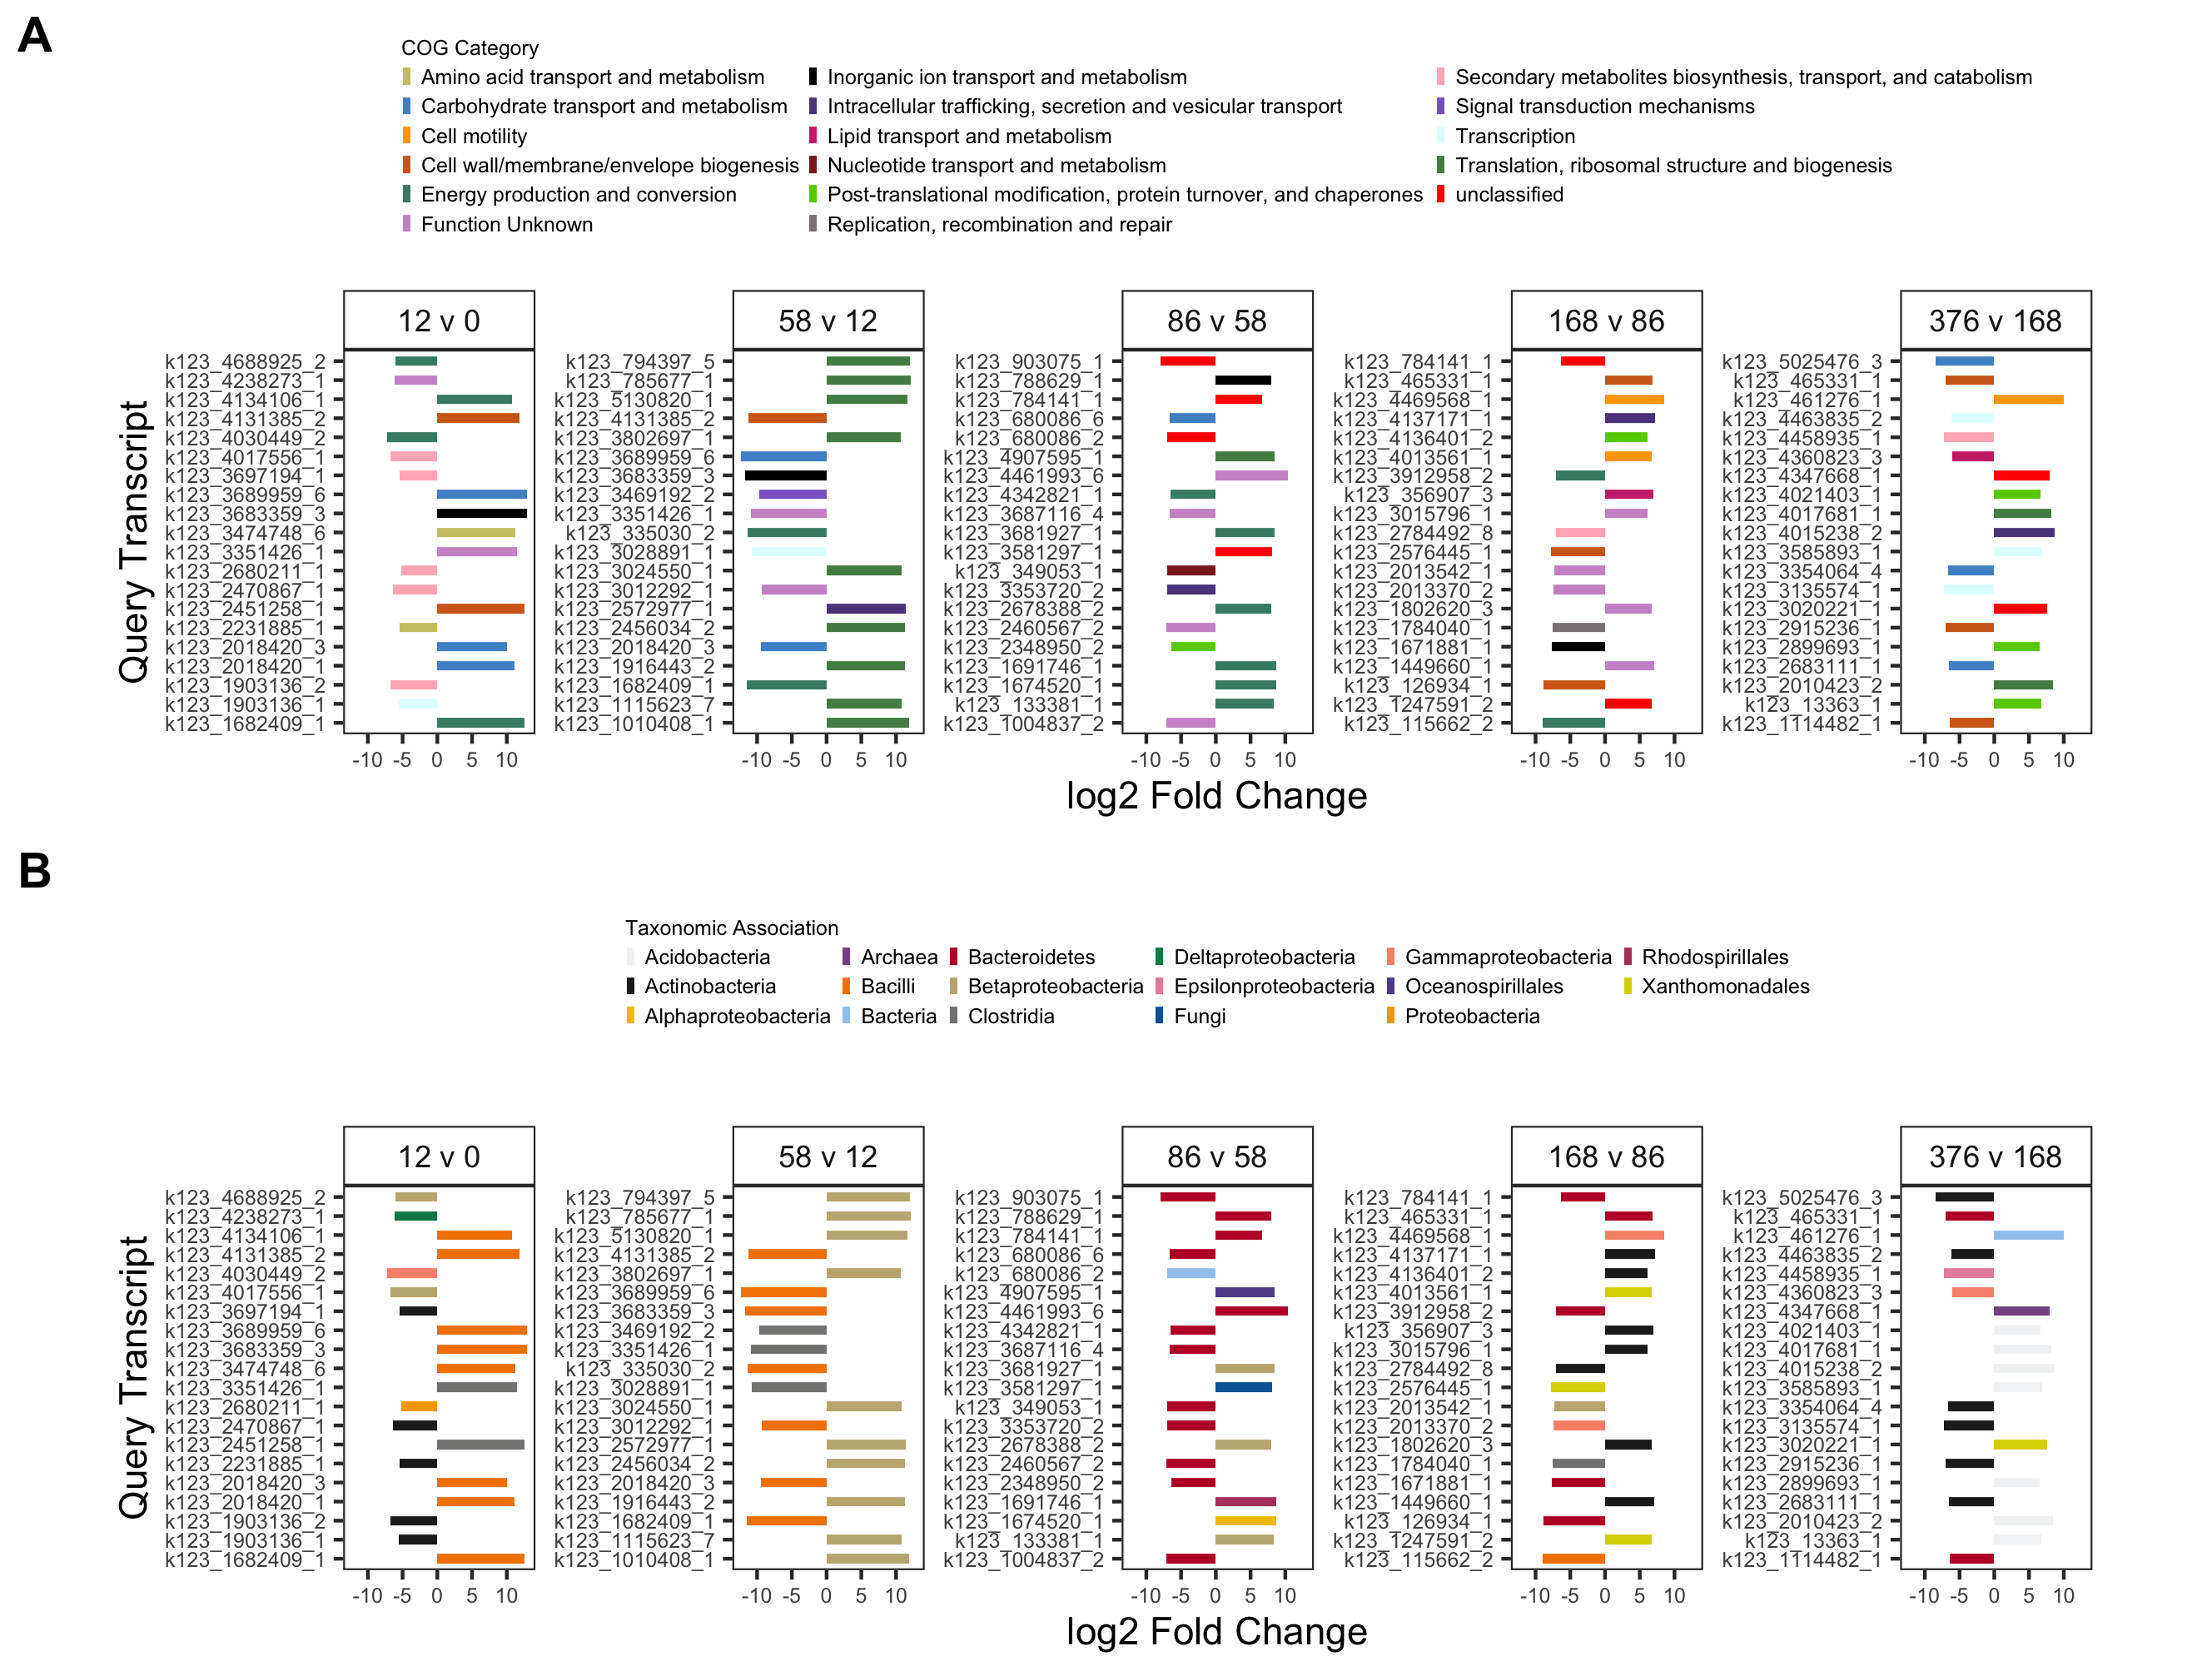
\includegraphics[keepaspectratio]{../../figures/Study.con_DE_top20_barplot.png}}

Expression of genes annotated with the COG categories cell
wall/membrane/envelope biogenesis, inorganic ion transport and
metabolism, and carbohydrate transport and metabolism increased
proporitionally from day 0 to 12. In contrast, expression of secondary
metabolite biosynthesis, transport, and catabolism genes decreased
during this period (Fig~\ref{fig-top-day-bar}A). Transcripts from
\emph{Bacilli} and \emph{Clostridia} increased, while transcripts from
\emph{Actinobacteria} decreased between study days zero and 12
(Fig~\ref{fig-top-day-bar}).

Between days 12 and 58, 90\% of the top 10 upregulated genes were
associated with the translation, ribosomal structure and biogenesis COG
and all were taxonomically associated with \emph{Betaproteobacteria}
(Fig~\ref{fig-top-day-bar}A,B). Many of these genes were annotated as
ribosomal protein large (RPL), involved in ribosomal binding. Genes
across multiple COG categories with taxonomic associations to
\emph{Bacilli} and \emph{Clostridia} decreased between study days 12 and
58, six of which were transcripts that previously increased between days
zero and 12 (Fig~\ref{fig-top-day-bar}B,
Supplementary Material~\ref{sup-t20-day-tbl}).

Multiple transcripts associated with the energy production and
conversion COG, as well as transcripts annotated with the COGs inorganic
transport and metabolism, and translation, ribosomal structure and
biogenesis, increased between days 58 and 86
(Fig~\ref{fig-top-day-bar}A). Two of the upregulated energy and
production and conservation transcripts were associated with cytochrome
c oxidase subunits in \emph{Betaproteobacteria}, while another was
annotated as \emph{hao}, encoding the enzyme hydroxylamine dehydrogenase
which is involved in conversion of hydroxylamine to nitrite during
nitrification (Supplementary Material~\ref{sup-t20-day-tbl}). Further
investigation into hydroxylamine dehydrogenase showed a significant
increase in \emph{hao} transcripts at day 86 followed by subsequent
decreases at days 168 and 376 (F = 4.183; \emph{p} = 0.02). This
increase corresponded to decreased soil ammonium levels and subsequent
accumulation of nitrate (Supplementary Material~\ref{sup-chem-plot}).
Half of the topmost downregulated genes between days 58 and 86 were not
assigned to a COG (\emph{i.e.}, unclassified) or were of unknown
function.

Differential expression comparing study days 86 with 168 and 168 with
376 identified genes across a variety of functional categories, with
many unclassified in the COG database or with unknown function
(Fig~\ref{fig-top-day-bar}A). Expression of carbohydrate transport and
metabolism genes associated with \emph{Bacilli} decreased between day
168 and 376. \emph{Acidobacteria} transcripts increased in
decomposition-impacted soils between study day 168 and 376, but were not
associated with any single COG category (Fig~\ref{fig-top-day-bar}B).

\subsection{Organic carbon metabolism}\label{organic-carbon-metabolism}

We expected to observe increased expression of lipid metabolizing genes
during active and advanced decomposition as microbes degraded lipids
deposited in the soil \citep{howard_characterization_2010}. Therefore,
we investigated changes in triacylglycerol lipase (enzyme commission
number: 3.1.1.3) gene transcription in our soils. Generally, lipase
transcripts decreased as decomposition progressed (HLM F = 6.564,
\emph{p} \textless{} 0.001), however we also observed a significant
interaction between study day and taxonomic annotation (F = 8.786;
\emph{p} \textless{} 0.001). Specifically, lipase gene transcripts
annotated as bacteria decreased with decomposition time (F = 10.392;
\emph{p} = 0.001), while fungal lipase transcripts increased, reaching a
maximum at study day 58 (F = 4.509; \emph{p} = 0.015)
(Fig~\ref{fig-lipase}).

% Place figure captions after the first paragraph in which they are cited.
\begin{figure}[!h]
\caption{{\bf Mean transcript abundance, in transcripts per million (TPM), of all bacterial (A) and fungal (B) triacylglycerol lipase (EC 3.1.1.3) genes over time.}
Black lines (A, B) report mean and standard deviation of TPM from three individuals (black line), while gold stars denote mean TPM in control soils. P-values are the result of ANOVAs where average TPM and study day are the dependent and independent variables, respectively, while letters are the result of post-hoc Tukey tests between decomposition timepoints. In B, bars show the relative abundance of the fungal classes \textit{Saccharomycetes}, \textit{Sordariomycetes}, and \textit{Eurotiomycetes}, reported in Taylor et al. (2024).}
\label{fig-lipase}
\end{figure}

\pandocbounded{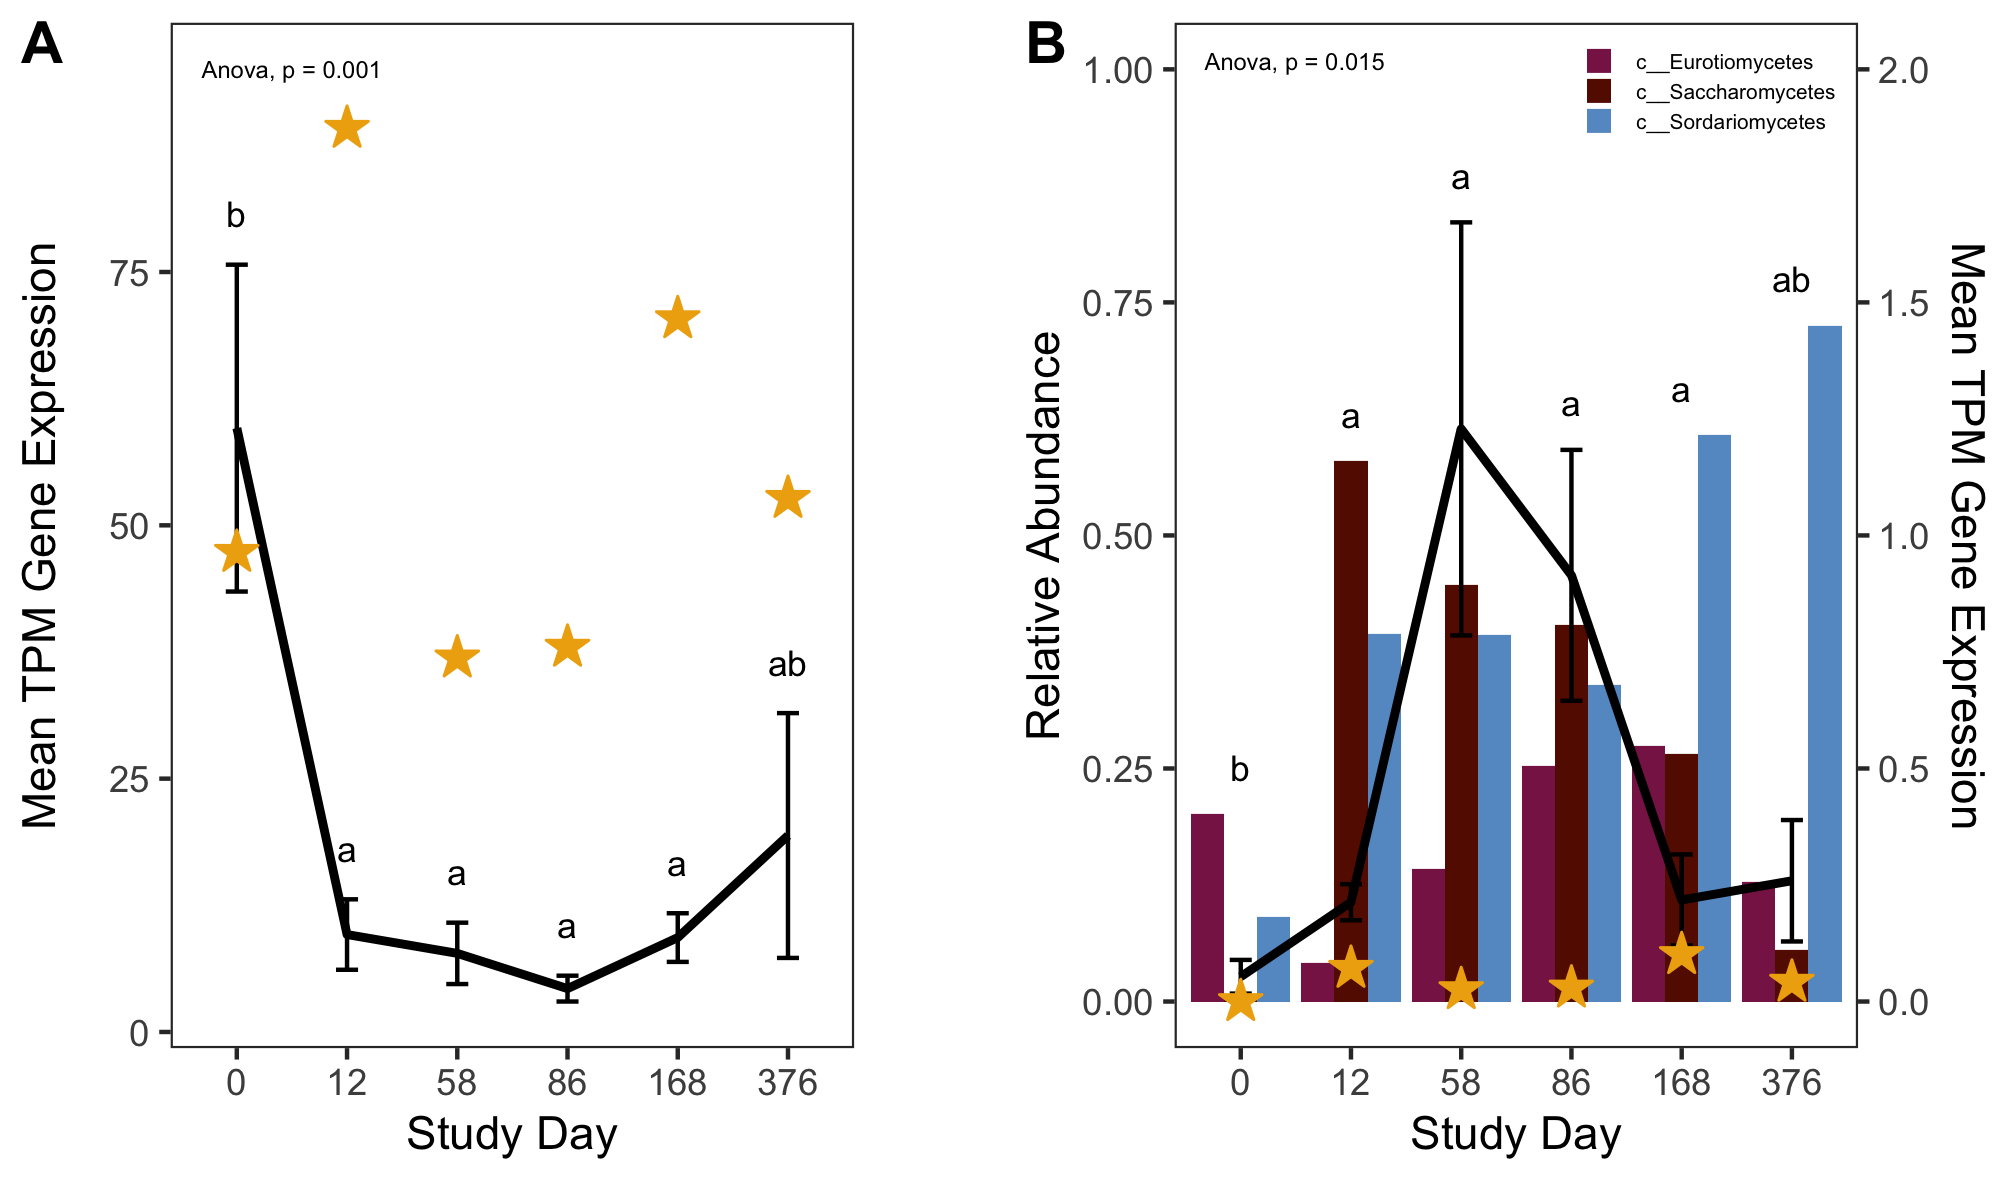
\includegraphics[keepaspectratio]{../../figures/Fig4.png}}

\subsection{Nitrogen- and sulfur compound
transformations}\label{nitrogen--and-sulfur-compound-transformations}

Expression of nitrogen cycling genes was impacted in response to human
decomposition. Due to the detection of hydroxylamine oxidoreductase
(\emph{hao}) transcripts in our differential expression analysis, and
our hypotheses predicting changes to nitrogen transformation processes,
the expression of genes encoding common enzymes involved in nitrogen
cycling (\emph{nifH}, \emph{nirB}, \emph{nirK}, \emph{norB},
\emph{nosZ}, \emph{nrfA}, \emph{nxrA}, and \emph{amoA}) were assessed
using their enzyme commission numbers (Fig~\ref{fig-n-genes}A,B).
\emph{nifH}, encoding a subunit of nitrogenase which is involved in
nitrogen fixation, displayed little to no changes in gene expression
between control and decomposition soils. Transcripts for two genes
encoding enzymes contributing to the last two steps of denitrification,
\emph{norB} (nitric oxide reductase) and \emph{nosZ} (nitrous oxide
reductase), increased between study days 12 and 86, and decreased at
study day 168 before increasing again at day 376. In contrast,
expression of genes encoding nitrate reductase, \emph{narG}, and
NO-forming nitrite reductase, \emph{nirK}, remained low until day 376
when transcripts for both genes increased. As noted above, expression of
\emph{hao}, encoding hydroxylamine dehydrogenase, increased at study day
86 before decreasing at remaining timepoints
(Fig~\ref{fig-top-day-bar}A, Fig~\ref{fig-n-genes}B). Expression of
\emph{amoA}, encoding a subunit of ammonia monooxygenase, and
\emph{nxrA}, encoding a subunit of nitrite oxidoreductase, which are
involved in nitrification, changed in response to decomposition.
\emph{amoA} transcripts initially decreased at day 12, remaining reduced
until study day 376. Similarly, abundance of genes that encode for
enzymes involved in dissimilatory nitrate reduction, \emph{nirB}, and
\emph{nrfA}, was low for the first 168 days, with \emph{nrfA} expression
increasing at day 376 (Fig~\ref{fig-n-genes}B).

% Place figure captions after the first paragraph in which they are cited.
\begin{figure}[!h]
\caption{{\bf Mean gene expression, in transcripts per million (TPM), of commonly used marker genes for enzymes involved in nitrogen cycling over time in controls (A) and decomposition (B) soils.}
Data in B represent mean and standard deviation of TPM from three individuals.}
\label{fig-n-genes}
\end{figure}

\pandocbounded{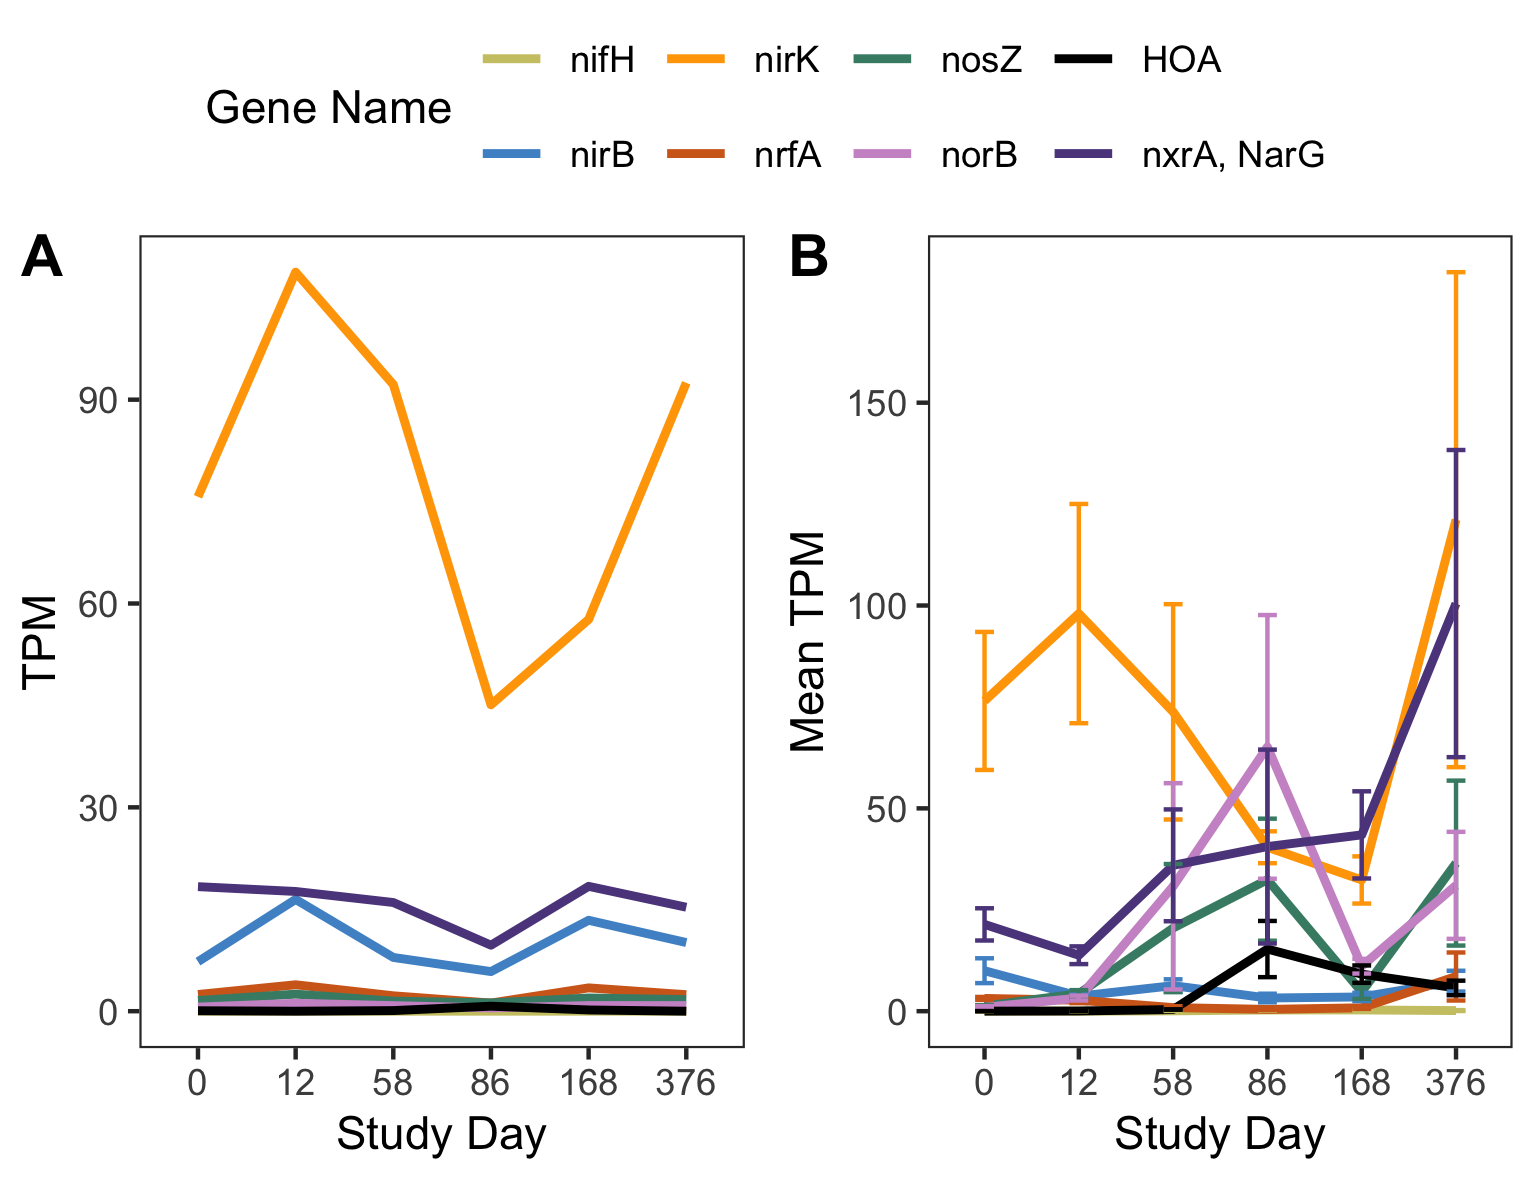
\includegraphics[keepaspectratio]{../../figures/Fig5.png}}

Expression of genes involved in metabolism of nitrogen and
sulfur-containing compounds were also impacted by human decomposition.
Specifically, four of the top ten genes whose expression decreased at
day 12 were related to taurine metabolism, with their annotations
associated with \emph{tauD}, encoding taurine dioxygenase.
(Supplementary Material~\ref{sup-t20-day-tbl}). Further investigation
into \emph{tauD} showed that mean expression of these genes decreased
steadily over one year, beginning at day 12 (Fig~\ref{fig-taud-bsh}B);
however, \emph{tauD} expression in response to human decomposition was
variable across taxonomic associations. Most \emph{tauD} transcripts
were associated with \emph{Gammaproteobacteria}, \emph{Actinobacteria},
\emph{Betaproteobacteria}, \emph{Alphaproteobacteria}, and fungi. While
a majority of the \emph{tauD} gene queries displayed reduced expression
over time, expression of fungal-associated and a few
\emph{Betaproteobacteria}-associated \emph{tauD} genes increased at day
58 (Supplementary Material~\ref{sup-taud-tax}). Sources of taurine in
the human body include taurine absorbed from the diet and taurine
produced from anaerobic microbial deconjugation of bile salts via bile
salt hydrolase (BSH) enzymes \citep{urdaneta_interactions_2017}.
Therefore, we examined expression for genes encoding BSH enzymes in
decomposition soils. Expression of these genes was elevated at days 12,
58, and 86 before converging toward pre-decomposition levels at days 168
and 376 (Fig~\ref{fig-taud-bsh}A). Hierarchical liner mixed effects
(HLM) models showed that both \emph{tauD} (HLM F = 7.356, \emph{p} =
0.002) and BSH (F = 13.768, \emph{p} \textless{} 0.001) gene expression
was significantly different over time (Fig~\ref{fig-taud-bsh}A,B).

% Place figure captions after the first paragraph in which they are cited.
\begin{figure}[!h]
\caption{{\bf Mean bile salt hydrolase, BSH, (A) and \textit{tauD}, taurine dioxygenase, (B) log2 normalized expression in controls (gold stars) and decomposition (boxplots) soils.}
Boxplots display the 25th and 75th quartiles and median log2 normalized values between all three individuals at each timepoint. ANOVA p-value is the result of a hierarchical linear mixed effects model accounting for repeated measures of each donor block, while letters denote the results of \textit{post-hoc} Tukey test.}
\label{fig-taud-bsh}
\end{figure}

\pandocbounded{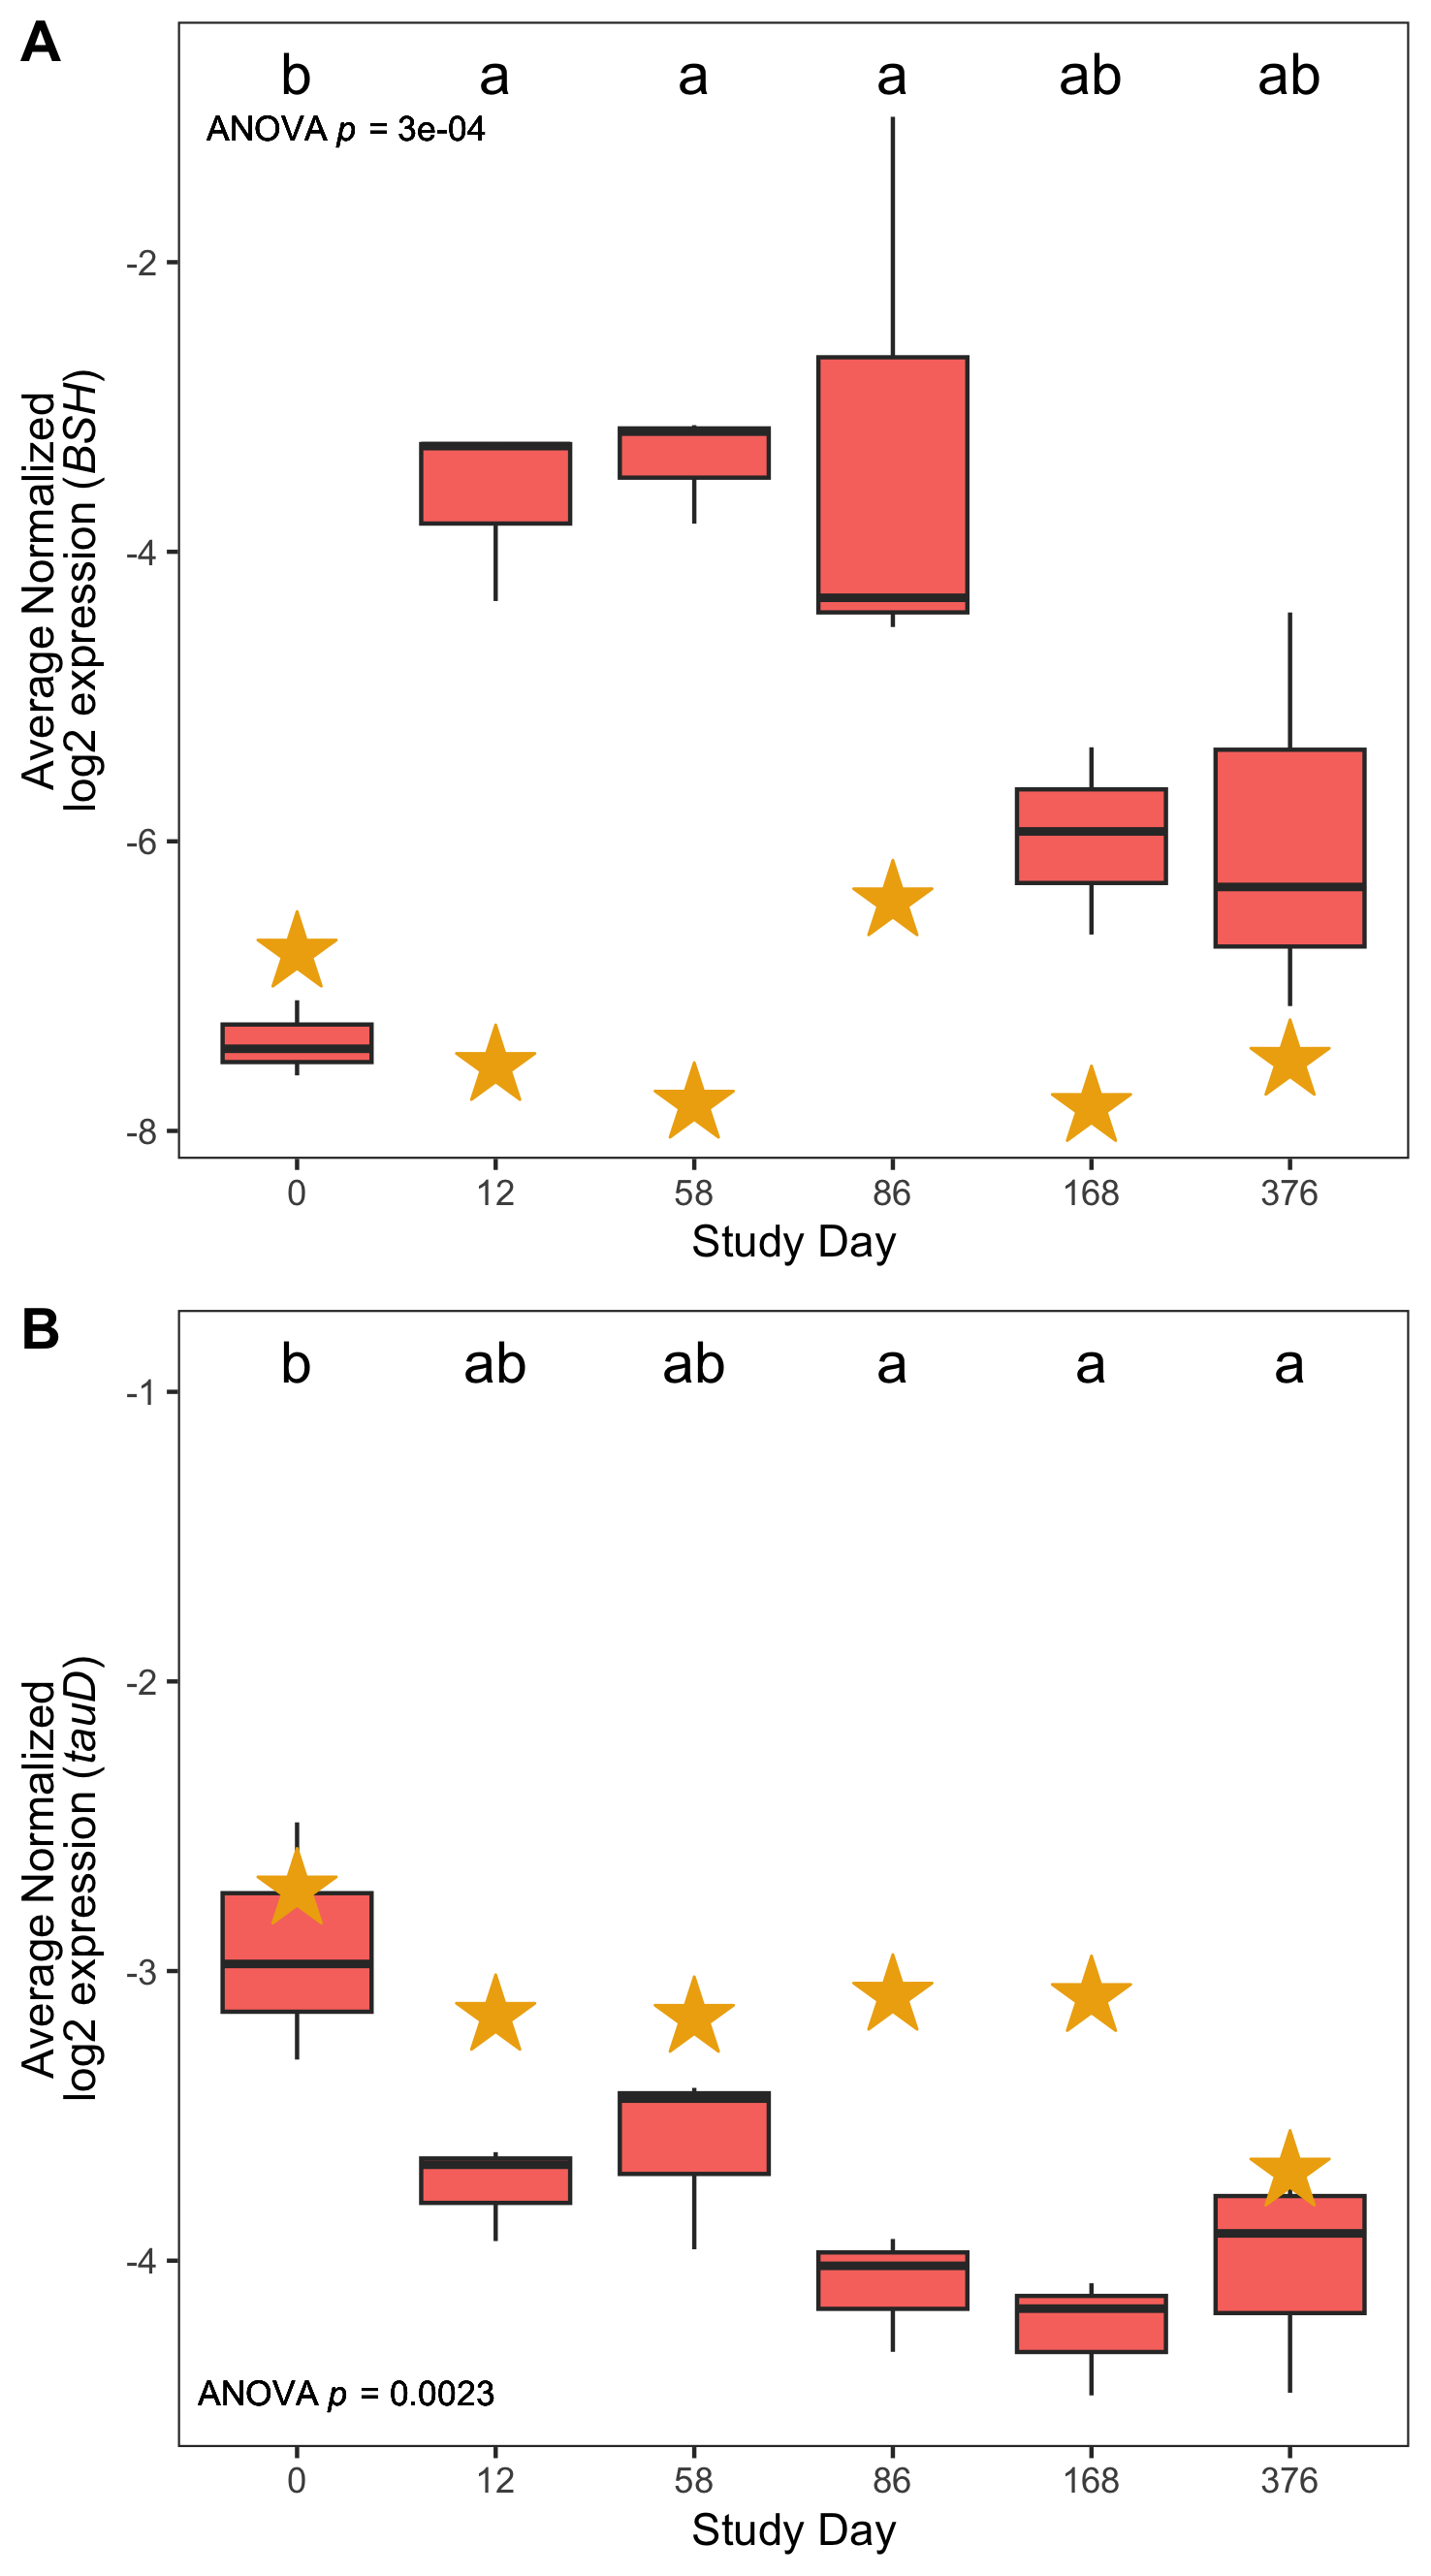
\includegraphics[keepaspectratio]{../../figures/tauD_bsh_nlog2.png}}

\section{Discussion}\label{discussion}

The goal of this study was to assess microbial gene expression in soils
responding to human decomposition. Metatranscriptomics were applied to
soil samples collected over one year from below three decomposing human
bodies. From this, we found that microbial gene expression reproducibly
shifted over time. Additionally, we showed that gene expression profiles
had not recovered to pre-decomposition conditions after one year.
Comparison of control and decomposition expression profiles revealed
that heat-shock proteins were elevated in response to decomposition. We
also described expression patterns between decomposition timepoints,
noting changes in functional gene categories at certain timepoints, in
particular with respect to lipid, nitrogen and sulfur metabolism.

\subsection{Decomposition impacted soil community gene expression, for
at least one
year}\label{decomposition-impacted-soil-community-gene-expression-for-at-least-one-year}

Gene expression profiles remained altered after one year of
decomposition. It is unclear if soil microbial communities, in terms of
gene expression profiles, have reached a new steady state as a result of
decomposition, or if they would eventually return to pre-decomposition
conditions. The soil pH, EC, NH\textsubscript{4}\textsuperscript{+},
NO\textsubscript{3}\textsuperscript{-}, and total nitrogen (TN)
exhibited differences (although not statistically significant) in these
soils following a year of decomposition, however bacterial and fungal
community structures, as assessed by rRNA amplicon libraries, were still
altered \citep{taylor_transient_2024}. This indicates that decomposition
can continue to structure microbial communities and impact their
function for extended periods of time. While nutrient pools and
communities both demonstrate less rapid change at later time points in
the study, there is no evidence suggesting an arrival at a steady-state
post-disturbance microbial community within our study. In some studies,
human decomposition can result in elevated carbon and nutrients (organic
nitrogen, ammonium, nitrate, and phosphate) for longer than a year
\citep{debruyn_carrion_2024}, suggesting decomposition events have
long-lasting effects on the local ecosystem. Together, this has
implications for terrestrial ecosystem processing (\emph{e.g.}, nutrient
cycling, emission of greenhouse gasses, etc.), as we show that
decomposition alters functional metabolism pathways within soil
microbial communities. It is clear that extended sample collections
beyond a single year are needed to address how long microbial
communities are effected, and whether there is a return to the original
state or some new altered community condition.

Bacteria, fungi, and archaea were all represented by expressed genes
throughout decomposition, suggesting that members of all three domains
have the potential to contribute to decomposition processes and nutrient
cycling. While a majority of annotated transcripts were identified as
bacterial, fungal transcripts were the second most abundant group.
Fungal transcripts made up almost half (\emph{e.g.}, seven of the top
fifteen) of the significantly differentially expressed genes associated
with decomposition-impacted soils. Additionally, with respect to
expression shifts between decomposition timepoints, fungal transcripts
were among the topmost upregulated genes at study day 86. This is not
surprising as fungi are key decomposers, involved in the degradation of
organic matter in terrestrial ecosystems
\citep{van_der_wal_thready_2013}. It was interesting to see an increase
in certain fungal transcripts, such as lipase, at study days 58 and 86
when soil oxygen began to recover. We would expect lipids to enter the
soil as tissues are broken down during decomposition, so we were
surprised to see bacterial lipase genes decrease during decomposition.
This suggests that microbial activity in decomposition soils may be
constrained by the changing chemical environment, potentially altered
oxygen levels in the case of bacterial lipase gene expression. Prior
work with these same soils showed that soil oxygen concentration was a
key driver of changes in both bacterial and fungal community composition
\citep{taylor_transient_2024}.

\subsection{Increased stress responses during
decomposition}\label{increased-stress-responses-during-decomposition}

Soil microbial communities expressed stress response genes in response
to human decomposition. Differential expression analysis identified
increased expression of multiple heat shock proteins associated with the
taxa \emph{Xanthomonadales}, \emph{Actinobacteria}, and fungi. Upon
further investigation, expression of these genes increased through day
58 and remained high for the remainder of the year. Soil temperature was
elevated relative to controls between study days 8 and 80, with maximum
temperatures \textgreater40°C, while soil electrical conductivity
increased up to 663 \textmu S/cm (16X higher than background) through
day 58 before slowly decreasing through the remainder of the study. Soil
electrical conductivity correlates with ionic strength and can be an
indicator of increased salinity \citep{essington_soil_2015}. With regard
to vertebrate decomposition, early elevated conductivity in impacted
soils is attributable to sodium (Na), potassium (K), and ammonium
(NH\textsubscript{4})
\citep{keenan_mortality_2018, fancher_evaluation_2017, quaggiotto_dynamic_2019, taylor_soil_2023, taylor_transient_2024}.
As a result, we would expect these microbes to be experiencing both heat
and osmotic stress during this period. Prior work has observed increased
heat shock gene expression during salt stress in paddy soils
\citep{peng_short-term_2017} and the presence of both heat and osmotic
stress genes in desert soils along a salt gradient
\citep{pandit_snapshot_2015}, suggesting saline conditions can alter the
expression of heat and/or osmotic stress genes. In our study we observed
the stress response within soil microbial communities was stimulated
during human decomposition. At this time, however, it is unclear if
expression of these genes is in response to heat stress alone, or in
combination with osmotic stress.

\subsection{Increased expression of fungal lipase genes during
decomposition}\label{increased-expression-of-fungal-lipase-genes-during-decomposition}

Human fat tissue contains lipids that are broken down during
decomposition. Therefore, we assessed expression of triacylglycerol
lipase genes in decomposition soils. Our results show that expression of
triacylglycerol lipase genes was altered in response to decomposition,
and these shifts differed between bacterial and fungal transcripts.
Specifically, bacterial triacylglycerol lipase transcripts decreased in
response to decomposition, while fungal triacylglycerol lipase
transcripts increased. Further, expression of these genes corresponded
to changes in relative abundance of the fungal classes
\emph{Saccharomycetes}, \emph{Sordariomycetes}, and
\emph{Eurotiomycetes} \citep{taylor_transient_2024}. These fungi have
been previously associated with decomposition soils
\citep{metcalf_microbial_2016, fu_fungal_2019} and are known to contain
triacylglycerol lipase genes in their genomes
\citep{dujon_genome_2004, haridas_genome_2013}, suggesting that they
play a role in lipid degradation in decomposition soils.

Our observation of an overall decrease in triacylglycerol lipase
transcripts contrasts with previous work by Howard et al.~(2010)
\citep{howard_characterization_2010}, who observed increased gene copy
number of Group 1 lipase genes via qPCR during swine decomposition.
Fatty acid composition differs in human compared to pig tissue
\citep{notter_initial_2009}, potentially altering the lipids profile
available for microbes, leading to differences in decomposition products
within the soil \citep{debruyn_comparative_2021}. These products can
then directly or indirectly alter community composition and/or activity
of functional proteins via substrate availability or the chemical
environment. Further, decomposition of humans and pigs resulted in
increased pH in soils below pigs, and decreased pH below humans
\citep{debruyn_comparative_2021}. Altered pH and soil chemistry could
result in a different functional potential and/or gene expression in
decomposition-impacted soils. Many triacylglycerol lipases have a pH
optimum that is neutral to basic
\citep{kok_characterization_1995, hasan_influence_2006, zouaoui_production_2012},
so cells may be decreasing expression under acidic conditions in human
decomposition soils. Availability of lipid species and changes to pH may
select for taxa that favor these substrates/pH conditions; for example,
Mason et al.~(2022) \citep{mason_body_2022} suggested the abundance of
the fungal taxa \emph{Saccharomycetes} was related to antemortem BMI due
to relative proportions of fat and muscle tissue.

\subsection{Evidence for phased denitrification and
nitrification}\label{evidence-for-phased-denitrification-and-nitrification}

The human body is a concentrated source of nitrogen that is released
into the surrounding soil during decomposition. Expression of common
marker genes for nitrogen cycling was altered in decomposition soil and
suggested nitrogen transformations during human decomposition are driven
by soil oxygen concentrations with hydroxylamine as an important
intermediate. We observed low or reduced expression of the nitrification
genes \emph{nxrA} and \emph{amoA} between days 12 and 86, during a
period when oxygen was reduced to 39\% - 85\%. This was concomitant with
an accumulation of ammonium, which reached a maximum on day 12, and low
nitrate conditions indicating that nitrification was inhibited. This
period of reduced soil oxygen constraining nitrification was also
described in a decomposition experiment with beaver carcasses Keenan et
al.~(2018) \citep{keenan_mortality_2018}.

We observed increased gene expression for the enzyme hydroxylamine
dehydrogenase (HAO) at day 86 while oxygen was reduced
(\textasciitilde85\%). This corresponded to simultaneous increases in
expression of genes encoding nitric oxide reductase (\emph{norB}) and
nitrous oxide reductase (\emph{nosZ}). Traditionally HAO has been
thought to process hydroxylamine to nitrite during nitrification, while
NorB and NosZ are enzymes involved in the last two steps of
denitrification converting nitric oxide (NO) to dinitrogen gas
(N\textsubscript{2}). However, recent work suggested hydroxylamine can
be converted to nitric oxide (NO), and can interact with multiple phases
of the nitrogen cycle \citep{soler-jofra_hydroxylamine_2021}. Even
though \emph{amoA} expression was shown to decrease during reduced
oxygen conditions, \emph{amoA} transcripts were still present and likely
able to convert ammonium to hydroxylamine as soil oxygen was not
completely depleted during decomposition. Additionally, a previous study
reported that the growth of the ammonia oxidizing bacteria
\emph{Nitrosomonas europaea} under anoxic conditions lead to
accumulation of hydroxylamine in a chemostat bioreactor
\citep{yu_nitrosomonas_2018}, suggesting anaerobic ammonium oxidation
(anammox) may also be occurring in decomposition soils. However, we did
not observe increases in \emph{nirK} expression, which might suggest
conversion of nitrite to NO for use in the anammox pathway. NO produced
via HAO activity may be used for anammox in these soils; however, the
role of hydroxylamine as an intermediate in anammox is still debated
\citep{soler-jofra_hydroxylamine_2021}. Therefore, our current
hypothesis is that hydroxylamine accumulates under anaerobic conditions
during decomposition, which can then be converted to NO by HAO. This NO
would then be present for anaerobic denitrifying bacteria to convert to
nitrous oxide (N\textsubscript{2}O) by NorB and finally to
N\textsubscript{2} by NosZ. Keenan et al.~(2018)
\citep{keenan_mortality_2018} noted a brief increase in
N\textsubscript{2}O emissions, which suggests denitrification was
occurring during this phase of reduced soil oxygen concentrations.

As soils fully reoxygenated by day 168, we observed increased expression
of genes encoding enzymes involved in aerobic nitrification, \emph{amoA}
and \emph{nxrR}. Nitrification is an oxygen-dependent process which
would convert accumulated ammonium to nitrate; the increase in nitrate
concentrations may then serve as a substrate for denitrification. We
observed increased expression of marker genes encoding all four enzymes
in the complete dissimilatory denitrification pathway (\emph{narG},
\emph{nirK}, \emph{norB}, and \emph{nosZ}) at day 376. Increased
expression of nitrification and denitrification marker genes is
consistent with the accumulation of nitrite, nitrate, and
N\textsubscript{2}O after oxygen is reintroduced to soils described in
Keenan et al.~(2018)
\citep{keenan_mortality_2018, debruyn_carrion_2024}. Together, gene
expression patterns in our study provide further insight into nitrogen
transformations in during vertebrate decomposition, suggesting an
important role of hydroxylamine.

\subsection{Increased expression of bile salt
hydrolases}\label{increased-expression-of-bile-salt-hydrolases}

Sulfur is present in various organic molecules, including taurine, a
sulfur- and nitrogen-rich compound involved in bile acid formation
\citep{urdaneta_interactions_2017}. Taurine in the human body can be
absorbed from the diet or synthesized in the liver
\citep{seidel_taurine_2019}. However, taurine is also produced as a
byproduct of the deconjugation of bile salts via bile salt hydrolases
(BSHs) present in the anaerobic gut taxa \emph{Lactobacillus} and
\emph{Clostridium} \citep{urdaneta_interactions_2017}. We observed
increased expression of genes encoding BSH enzymes between days 12 and
86. Given that increased expression of BSH genes corresponded to the
beginning of active decomposition, when decomposition products were
observed to enter the soil, and the period of reduced dissolved oxygen
in our study, it is likely that taurine accumulation is the result of
BSH enzyme activity by anaerobic microorganisms. While we did not
measure taurine concentrations in the present study, our results
correspond to previous decomposition studies that report accumulation of
taurine in various organs and body regions
\citep{mora-ortiz_thanatometabolomics_2019, locci_1h_2019, zelentsova_post-mortem_2016}
and soils
\citep{debruyn_comparative_2021, hoeland_katharina_investigating_2021}
during decomposition via metabolomics, and increased relative abundance
of \emph{Clostridium }and \emph{Lactobacillus} within the body
\citep{javan_human_2016, javan_cadaver_2017, debruyn_postmortem_2017}
and in decomposition soils \citep{cobaugh_functional_2015} via DNA
sequencing methods, including in these soils
\citep{taylor_transient_2024}.

Taurine can be metabolised through desulfurization via the
\textalpha-ketoglutarate-dependent enzyme taurine dioxygenase (TauD).
Specifically, this enzyme, encoded by the gene \emph{tauD}, converts
2-oxoglutarate and taurine to produce aminoacetaldehyde, succinate,
sulfite, and CO\textsubscript{2} \citep{cook_metabolism_2006}. Succinate
and sulfite from this reaction can then be used for the citric acid
cycle and sulfur metabolism, respectively. Given increased BSH
expression in our study and reported taurine accumulation in others, we
would expect taurine to be present for microbial metabolism by TauD.
However, we observed a general decrease in \emph{tauD} expression
between days 12 through 376. This trend was driven by reduced expression
of \emph{tauD} transcripts associated with \emph{Proteobacteria},
\emph{Gammaproteobacteria}, and \emph{Actinobacteria} whose relative
abundance have been shown to remain consistent or increase during human
decomposition \citep{cobaugh_functional_2015}, suggesting that
\emph{tauD} expression is downregulated under decomposition conditions.
However, we noted that expression of \emph{tauD} genes associated with
fungi and a few \emph{Betaproteobacteria} displayed increased
representation at day 58, corresponding to increased expression of bile
salt hydrolases (BSH) between days 12 and 86. The reduction in
\emph{tauD} expression may be due to increased sulfur availability. We
did not measure sulfur species in this experiment; however, others have
observed increased sulfur concentrations in decomposition-impacted soils
\citep{aitkenhead-peterson_mapping_2012, taylor_soil_2023, debruyn_carrion_2024}.
Thus, sulfur scavenging pathways such as taurine desulfurization by TauD
\citep{kertesz_riding_2000}, whose genes are expressed under
sulfur-limiting conditions, likely display reduced expression under
sulfur replete conditions. Additionally, taurine may be processed
through other pathways. For example, taurine can be deaminated by
taurine dehydrogenase to produce sulfite and acetyl-CoA for carbon
metabolism \citep{cook_metabolism_2006, bruggemann_enzymes_2004}.
Overall, our results suggest that human decomposition has potential
impacts on soil sulfur biogeochemistry through deposition of inorganic
(sulfate) and organic (sulfur-containing amino acids) sulfur compounds.

\section{Conclusion}\label{conclusion}

This study investigated soil microbial gene expression during human
decomposition. Metatranscriptomic analysis of soils from three human
individuals shows that decomposition impacted microbial community gene
expression profiles, exhibiting functional shifts over time for over one
year. This included altered expression of genes involved in lipid, N and
S metabolism as microbes processed the nutrient-rich tissues of the
human body. Additionally, we noted that functionality within
decomposition-impacted soils was still affected after one year and had
not returned to starting or background conditions. Together, these
results show that vertebrate decomposition has lasting impacts on local
soil ecosystems, including soil microbial communities. These results
have important implications for understanding biogeochemical changes due
to vertebrate mortality events in terrestrial ecosystems.

\section{Materials and Methods}\label{materials-and-methods}

\subsection{Study design}\label{study-design}

In February 2018, three deceased male human subjects (hereafter,
``donors'') were placed supine on the soil surface at the University of
Tennessee Anthropology Research Facility (ARF) and allowed to decompose.
Located in Knoxville, TN (35° 56' 28'' N, 83° 56' 25'' W) the ARF is a
roughly 2-acre outdoor facility dedicated to studying human
decomposition \citep{keenan_spatial_2018}. The soils at the ARF are
comprised of the Loyston-Talbott-Rock outcrop (LtD) and Coghill-Corryton
(CcD) complexes. LtD soils are a silty clay loam and channery clay
overlaying lithic bedrock, while CcD soils are comprised of clay from
weathered quartz limestone
\citep{keenan_spatial_2018, taylor_transient_2024}. A site that had not
been previously exposed to decomposition was used for this study.

The decomposition field experiment is fully described in Taylor et
al.~(2024) \citep{taylor_transient_2024}. Briefly, experiments were
conducted in a block design, where each block consisted of one
decomposition site and one control site \citep{taylor_transient_2024}.
In total three blocks, \emph{i.e.}, three donors paired with three
respective control sites, were included in the study. Each control site
was chosen in a manner to ensure their location was uphill and roughly 2
m away from decomposition sites \citep{taylor_transient_2024}. Donor
internal temperatures were recorded by probes located in the abdomen,
while ambient air temperatures were monitored via sensors located
roughly 50 cm above the soil surface. Soil temperature and salinity were
measured with sensors placed directly underneath each individual
(Decagon Devices, GS3) \citep{taylor_transient_2024}. Donor ages ranged
from 65 to 86 and were within 1 kg of each other with regard to weight
(90.7 to 91.6 kg); donor BMI varied between 27.7 to 29.6
\citep{taylor_transient_2024}.

\subsection{Sampling and
physiochemistry}\label{sampling-and-physiochemistry}

Decomposition of all subjects was observed for one year. During the
one-year study period, soils were sampled at 20 timepoints chosen to
correspond with morphological stages of decomposition as described by
\citep{payne_summer_1965}. Once advanced decay was reached, soils were
collected at intervals of 350 accumulated degree days (ADD), calculated
using ambient air temperatures, up to one year. All soil cores were
taken using a 1.9 cm (3/4 inch) diameter soil auger to a depth of 16 cm.
Soils were divided into two depth fractions: 0-1 cm (interface) and 1-16
cm (core) for the analyses reported in Taylor et al.~(2024)
\citep{taylor_transient_2024}; the entire 0 to 16 cm core was used for
this current study. Decomposition soils were taken from directly beneath
the cadavers, taking care to not re-sample the same location more than
once. At the time of sampling, soil dissolved oxygen was measured in
triplicate using an Orion Star™ A329 pH/ISE/Conductivity/Dissolved
Oxygen portable multiparameter meter (ThermoFisher)
\citep{taylor_transient_2024}.

A subset of 6 study timepoints were chosen for metatranscriptomics
analysis. Study days 0, 12, 58, 86, 168, and 376 were chosen as they
represented distinct morphological and soil biogeochemical stages during
decomposition. Study day 0 was chosen as a baseline sample prior to
cadaver placement. Study day 12 was the start of active decomposition
and corresponded to maximum soil ammonium concentrations and minimum
soil oxygen (approximately 39\%). Study day 58 was chosen as this sample
represented the pH minimum, and respiration and soil temperature were at
a maximum \citep{taylor_transient_2024}. Additionally, ammonium
concentrations began to decrease around day 58. Study day 86 was when
soil oxygen started to recover and nitrate levels began to increase.
Study day 168 was chosen as nitrate was at its maximum and soil
dissolved oxygen had returned to 99\%. Finally, day 376 was chosen to
represent the end of the study, 1 year since cadaver placement. Each
study day was represented by four soil samples for RNA extraction: one
pooled control sample which was a mix of the three control locations,
plus one sample from each of the three donors, yielding a total of 24
samples for this study.

Soil samples were transported back to the University of Tennessee
(Knoxville, TN) and processed within 24 hours of collection. Soils were
homogenized by hand to remove insect larvae, roots, rocks, and other
debris (\textgreater{} 2 mm). A subset of soils were used to measure pH,
electrical conductivity (EC), and evolved CO\textsubscript{2} as
described in Taylor (2024). Soil nitrogen species
(NH\textsubscript{4}\textsuperscript{+},
NO\textsubscript{3}\textsuperscript{-}) and total carbon (TC) and
nitrogen (TN) were measured in all soil samples as described in
\citep{taylor_transient_2024}. Reported values for soil physiochemistry
represent the full 16 cm core; estimated by summing interface and core
values reported by Taylor et. al, (2024) \citep{taylor_transient_2024}
in 1:16 and 15:16 ratios, respectively. Control reported here are means
of the three experimental controls that were unimpacted by
decomposition.

Roughly 10 g of soil was reserved for nucleic acid extraction, placed in
a 4 oz. Whirl-Pak\texttrademark~bag (Nasco), and flash frozen in liquid
nitrogen. All samples were stored at -80°C until further analysis.
Bacterial and fungal community composition was assessed via amplicon
sequencing of the 16S rRNA gene and ITS2 region as described in Taylor
et al.~(2024).

\subsection{RNA Extraction and
Sequencing}\label{rna-extraction-and-sequencing}

RNA was extracted from 2 g of soil using Qiagen's
RNeasy\textregistered~PowerSoil\textregistered~Total RNA kit.
Manufacturer's instructions were followed with a few modifications.
Soils became saline during decomposition; therefore, we followed the
manufacturer's suggestion and incubated all extracts at -20°C following
addition of solution SR4 (step 9) to decrease salt precipitation. All
RNA samples were resuspended in 40 \textmu l of Solution SR7. RNA
concentrations were assessed fluorometrically using the
Qubit\textregistered~RNA HS assay (catalog no. Q32852) with 1 \textmu l
of RNA. DNA contamination was removed by DNase treating RNA extracts
twice using Qiagen's DNase Max\textregistered~kit in 50 \textmu l
reactions. RNA concentrations were remeasured after DNase treatment. PCR
with V4 16S rRNA gene primers
\citep{apprill_minor_2015, parada_every_2016} was conducted using RNA
extracts as the template to confirm removal of all DNA prior to
sequencing. RNA aliquots were shipped to HudsonAlpha Discovery
(Huntsville, AL) for library preparation and RNA sequencing.
Dual-indexed libraries were prepared using the Illumina® Stranded Total
RNA prep with ribosomal RNA depletion via ligation with Ribo-Zero Plus.
Libraries were then pooled and sequenced on Illumina's NovaSeq 6000 v4
platform, resulting in demultiplexed fastq files for each sample.

\subsection{Bioinformatics}\label{bioinformatics}

Illumina sequencing of the 24 libraries yielded a total of 5,073,476,730
reads, or 2,536,738,365 paired reads, with a mean of 105,697,432 paired
reads per sample. Read quality control (QC) was conducted in KBase
\citep{arkin_kbase_2018} using Trimmomatic
\citep{bolger_trimmomatic_2014}. Paired fastq files were imported to
KBase through Globus. Poor quality reads were removed (4.7\% of all
reads), and adapters trimmed via Trimmomatic (v0.36) using default
settings and the TruSeq3-PE-2 adapter file, resulting in 4,834,123,062
total reads. After QC check with FastQC, trimmed libraries were exported
as fastq files from KBase through Globus. Remaining ribosomal RNA was
filtered using bbmap (maxindel = 20, minid = 0.93) from the Joint Genome
Institute's (JGI) bbtools suite \citep{bushnell_bbtools_2014}. Filtering
of ribosomal RNA further removed 7.3\% of reads, leaving 4,479,804,360
reads for assembly. Following this step, all non-ribosomal reads from
all 24 samples were merged into one file. Reads were then co-assembled
into contigs using the de novo assembler MEGAHIT (v1.2.9)
\citep{li_megahit_2015} (--12 --k-min 23, --k-max 123, --k-step 10).

Gene identification and annotation from co-assembled contigs was
performed using Prodigal \citep{hyatt_prodigal_2010} and eggNOG mapper
\citep{cantalapiedra_eggnog-mapper_2021}, respectively. Briefly, the DNA
fasta containing all contigs was submitted to Prodigal (v2.6.3) for
protein coding gene predication for a meta-sample (-p meta -f gff).
After co-assembly, a total of 6,257,674 gene calls were identified by
Prodigal. Next, predicated genes were functionally and taxonomically
annotated using eggNOG mapper (v2.1.6) using basic settings to perform a
diamond blastp search \citep{buchfink_sensitive_2021}. From this,
1,048,573 proteins were annotated by eggNOG-mapper (16.7\%). Most of the
annotated proteins were taxonomically annotated as bacteria (91.3\%),
followed by eukaryotes (7.6 \%), and archaea (0.81 \%). Of the 7.6\% of
eukaryotic proteins, 64.4\% (4.9\% of all proteins) were annotated as
fungi. For this study, genes of interest included all bacterial,
archaeal, and fungal proteins, therefore all non-fungal eukaryotic
proteins (32,004) were removed prior to downstream analysis. Transcript
counts for all genes of interest were obtained by mapping reads from
each respective sample to genes of interest obtained from co-assembly
using QIAGEN CLC Genomics Workbench 20.0
(https://digitalinsights.qiagen.com/). The percent of reads mapped to
genes of interest ranged from 21\% to 38\% between samples, with an
average of 31\% reads mapped. Gene counts were then combined in a single
file and used for downstream analyses in R.

\subsection{Differential Expression}\label{differential-expression}

Transcript counts from all samples were combined in a single workable
data file and imported into R for differential expression analysis using
the R packages edgeR \citep{robinson_edger_2010} and limma
\citep{smyth_limma_2005} following a modified pipeline by Phipson et
al.~(2020) \citep{phipson_differential_2020}. The transcript count table
was imported into R and converted to a DGElist object. Genes without
sufficient counts for statistical analysis were removed to increase
power using the edgeR function filterByExpr(), using study day as the
comparison group.

Raw counts were then log2 normalized and gene expression profiles
compared via multidimensional scaling (MDS) and hierarchical clustering.
Multidimentional scaling (MDS) was conducted using plotMDS() from the
limma package to assess differences between samples. MDS values were
extracted from the MDS object, and the first two dimensions plotted
using ggplot2 \citep{wickham_ggplot2_2016}. We also assessed the
relationship between gene expression profiles and changes in the soil
environment using canonical correspondence analysis (CCA). Environmental
variables of interest included decomposition time in accumulated degree
hours (ADH) based on ambient temperatures, ADH based on internal gut
temperatures, ADH based on soil temperatures, gravimetric moisture, pH,
electrical conductivity (EC), dissolved oxygen (DO), CO\textsubscript{2}
(\textmu mol gdw\textsuperscript{-1}), NH\textsubscript{4} (mg
gdw\textsuperscript{-1}), NO\textsubscript{3} (mg
gdw\textsuperscript{-1}), N \%, C \%, and CN ratio. First, permutational
multivariate analysis of variance (PERMANOVA) with adonis() (vegan
v2.6.7) \citep{oksanen_vegan_2024} was used to identify significant soil
parameters. Then the vegan functions cca() and scores() were applied to
run the CCA and extract scores, respectively. Scores for the first two
dimension were plotted using ggplot2, with loadings extracted from the
CCA biplot.

For differential expression analysis, raw filtered reads were normalized
using edgeR's trimmed mean of M values (TMM) normalization using the
function calcNormFactors(). TMM normalized reads were then log2
transformed using limma's voom() and differential expression assessed.
Empirical Bayes shrinkage was used correct to p-values for false
discovery rates. The topmost up and down regulated genes for each
comparison, determined by log2 fold change and adjusted p-values, were
then reported. Expression of certain genes were assessed after
performing transcripts per million (TPM) normalization and statistical
analyses with a combination of analysis of variance (ANOVA) and post-hoc
Tukey tests. ANOVA across all timepoints were applied to hierarchical
linear mixed effects models to account for repeated sampling within each
donor block.

\section{Data availability}\label{data-availability}

Raw RNA sequence files from the Illumina Novaseq are available at the
National Center for Biotechnology Information's (NCBI) Sequence Read
Archive (SRA) as a part of
\href{https://www.ncbi.nlm.nih.gov/bioproject/PRJNA1066312/}{BioProject
PRJNA1066312} under BioSample accession numbers
SAMN45195141-SAMN45195164. Additional datasets supporting the
conclusions of this article are available on
\href{https://github.com/amason30/Mason_MetaT_XXX_2024}{GitHub}.

\section{Code availability}\label{code-availability}

The code used for analysis and to generate figures are available on
\href{https://github.com/amason30/Mason_MetaT_XXX_2024}{GitHub}.

\section{References}\label{references}

\renewcommand{\bibsection}{}
\bibliography{bibliography.bib}

\section{Acknowledgements}\label{acknowledgements}

We would like to thank the Forensic Anthropology Center at the
University of Tennessee-Knoxville for their help in setting up field
experiments. We would like to thank Mary Davis for her help in managing
the field site and helping to obtain donors for this work. This research
was funded by a National Institute of Justice Award
(DOJ-NIJ-2017-R2-CX-0008) to LST and JMD.

\section*{Supplementary Information}\label{supplementary-information}
\addcontentsline{toc}{section}{Supplementary Information}

\begin{supplemental}

\centering{

\pandocbounded{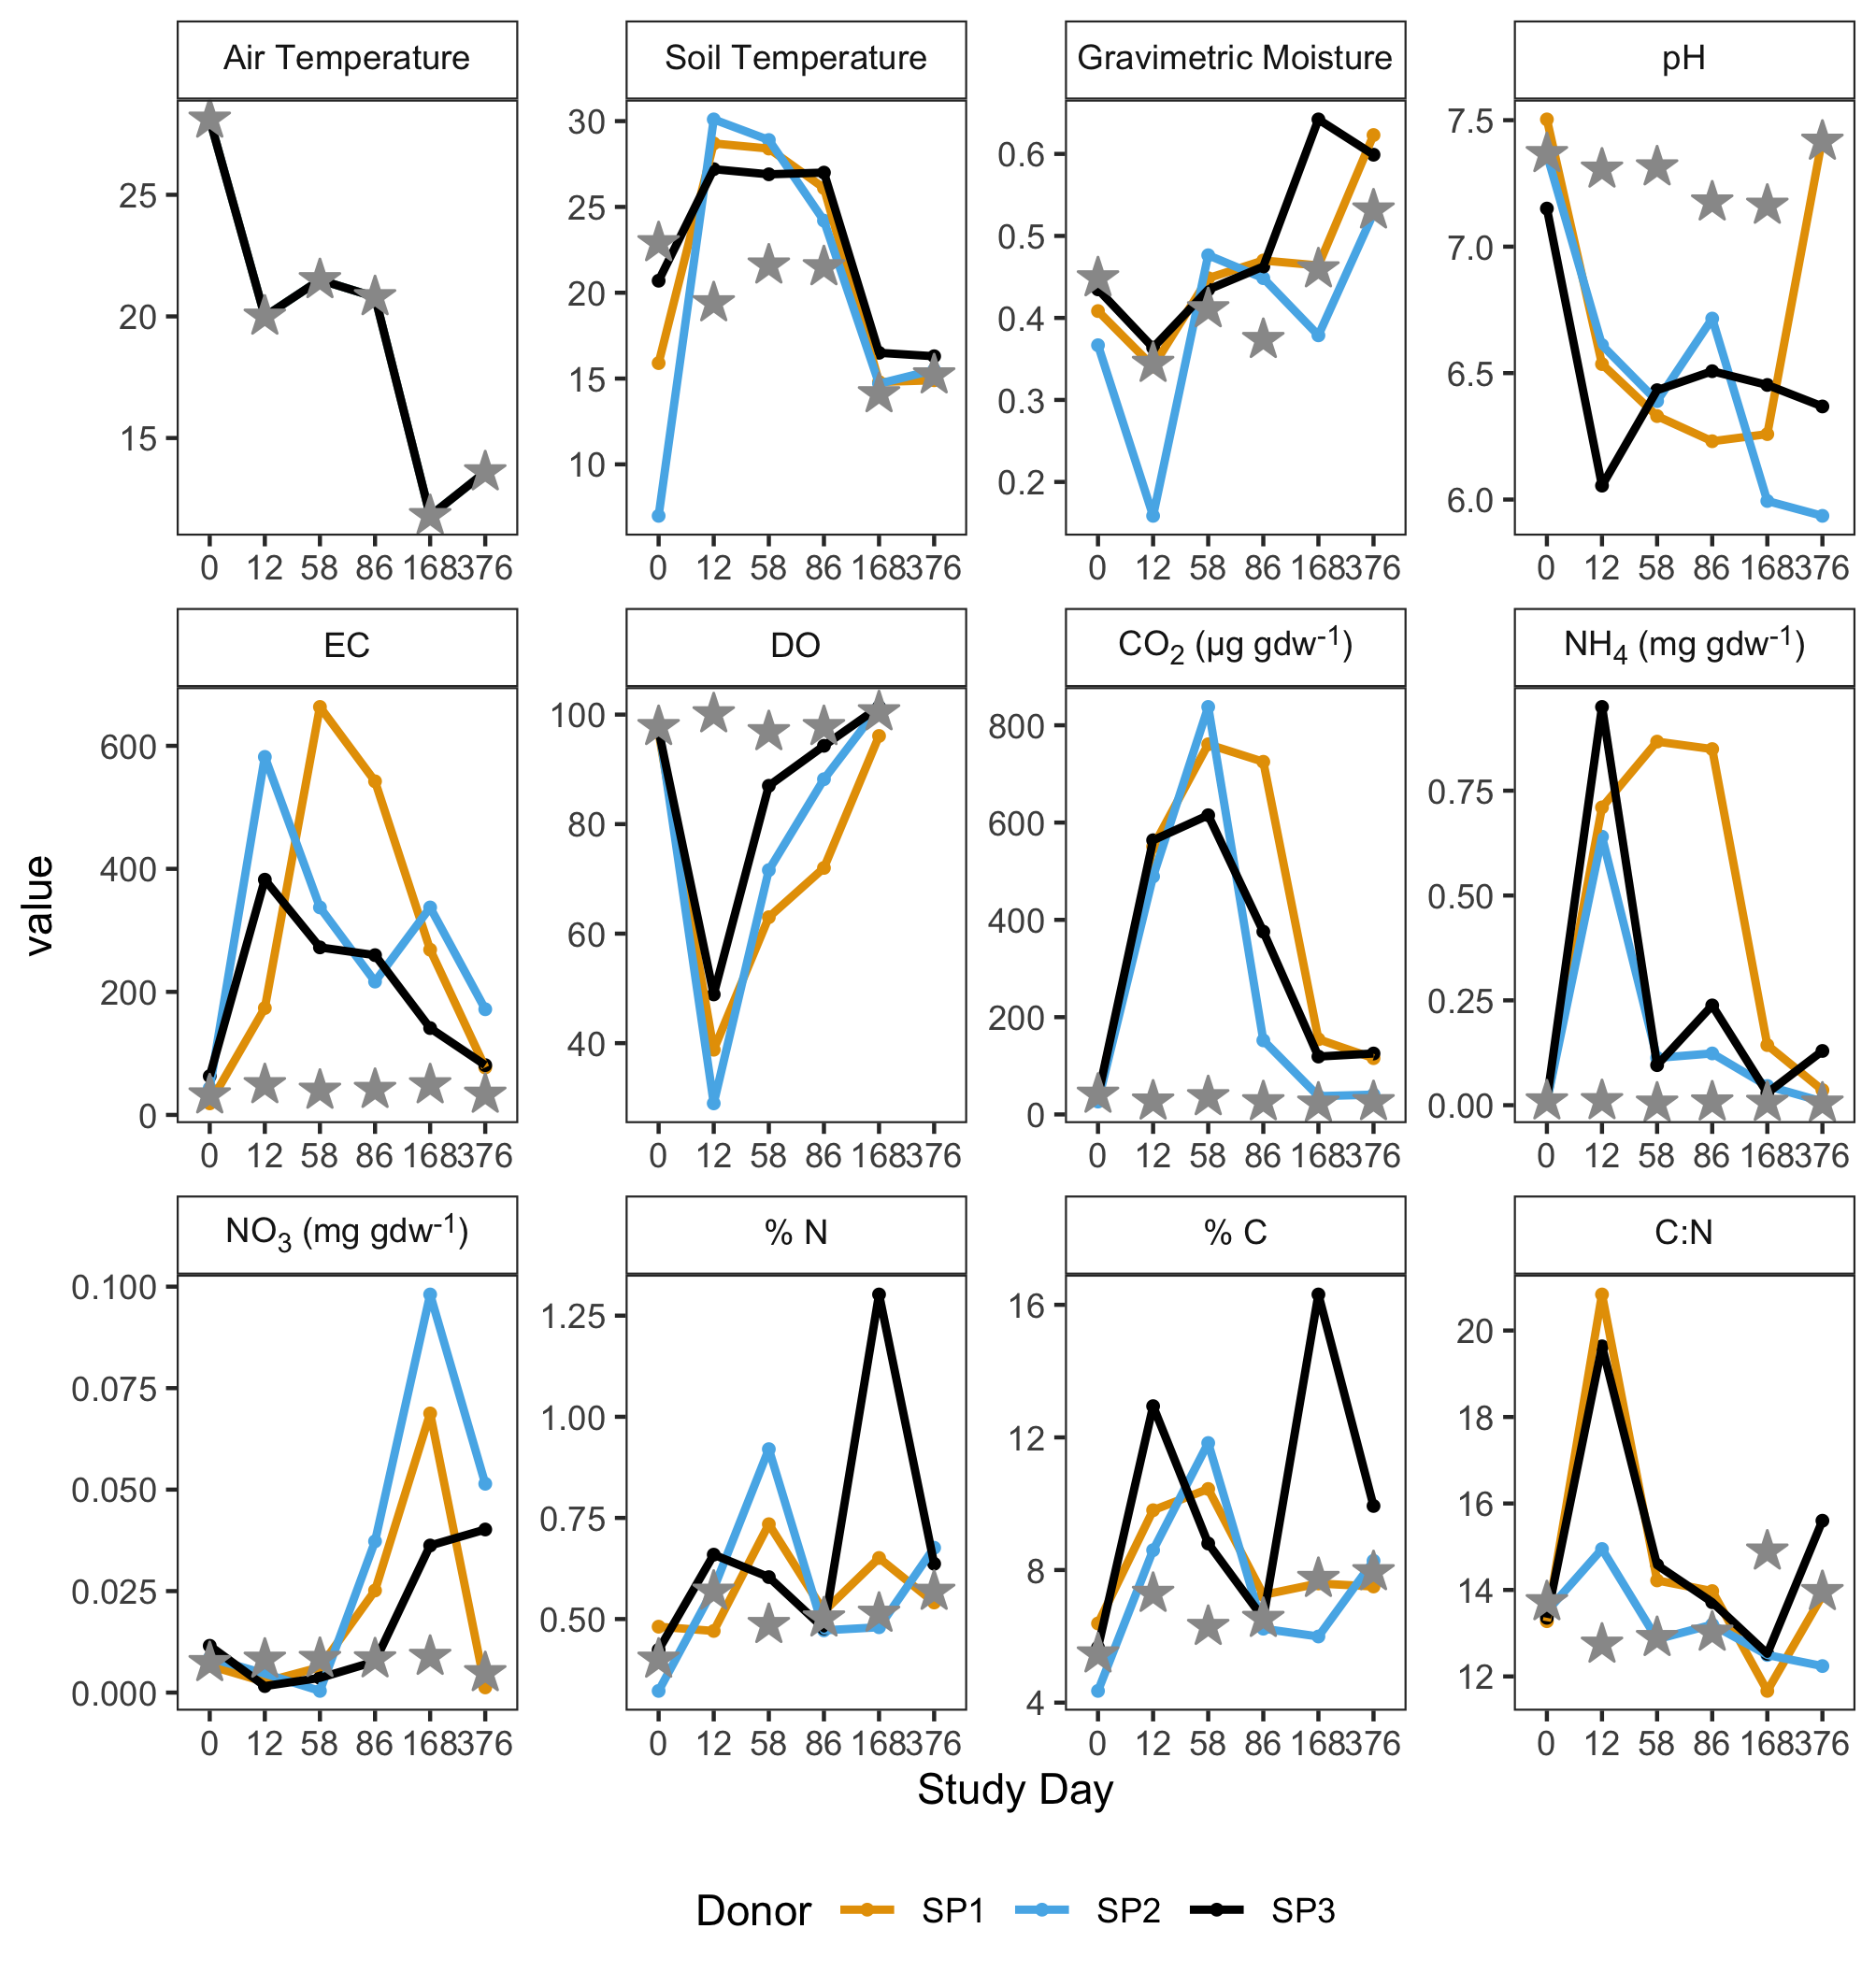
\includegraphics[keepaspectratio]{../../figures/soilchem_summary.png}}

}

\caption{\label{sup-chem-plot}Figure S1. Soil physiochemical parameters
in decomposition soils during the one-year study. Data is shown for each
individual donor: SP1 (gold), SP2 (blue), and SP2 (black). Values for
the full 16 cm core samples were estimated by summing values interface
(0-1 cm) and core (0-16 cm) reported by Taylor et al, (2024) in 1:16 and
15:16 ratios, respectively. Controls reported here are means of three
experimental controls that were unimpacted by decomposition and are
represented by stars.}

\end{supplemental}%

\begin{supplemental}

\centering{

\pandocbounded{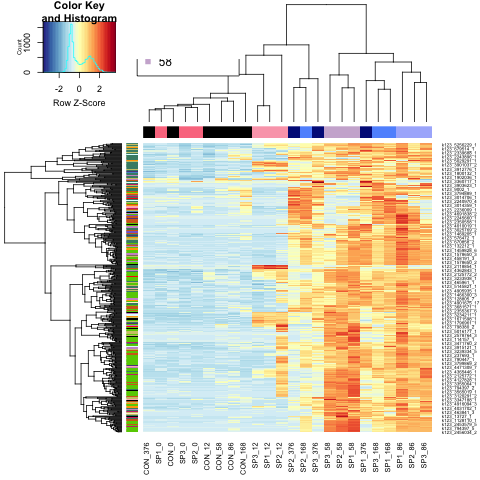
\includegraphics[keepaspectratio]{../../figures/Fig_S2.png}}

}

\caption{\label{sup-heatmap-plot}Figure S2. Hierarchical clustering
heatmap showing the log counts per million (CPM) of the top 500 most
variable genes across samples. Variable genes were determined by
selecting genes with the highest variance in gene expression. Samples
are clustered along the x-axis using Euclidean distances between samples
and colored by study day.}

\end{supplemental}%

\begin{supplemental}

\centering{

Table S1. Permutational analysis of variance (PERMANOVA) results
identifying significant environmental parameters which explain some of
the variation in soil gene expression profiles. Environmental parameter
data is from Taylor et al.~(2024). Variables with p \textless{} 0.05 are
indicated in bold.

}

\caption{\label{sup-tbl-cca-panova}}

\end{supplemental}%

\begin{supplemental}

\centering{

\pandocbounded{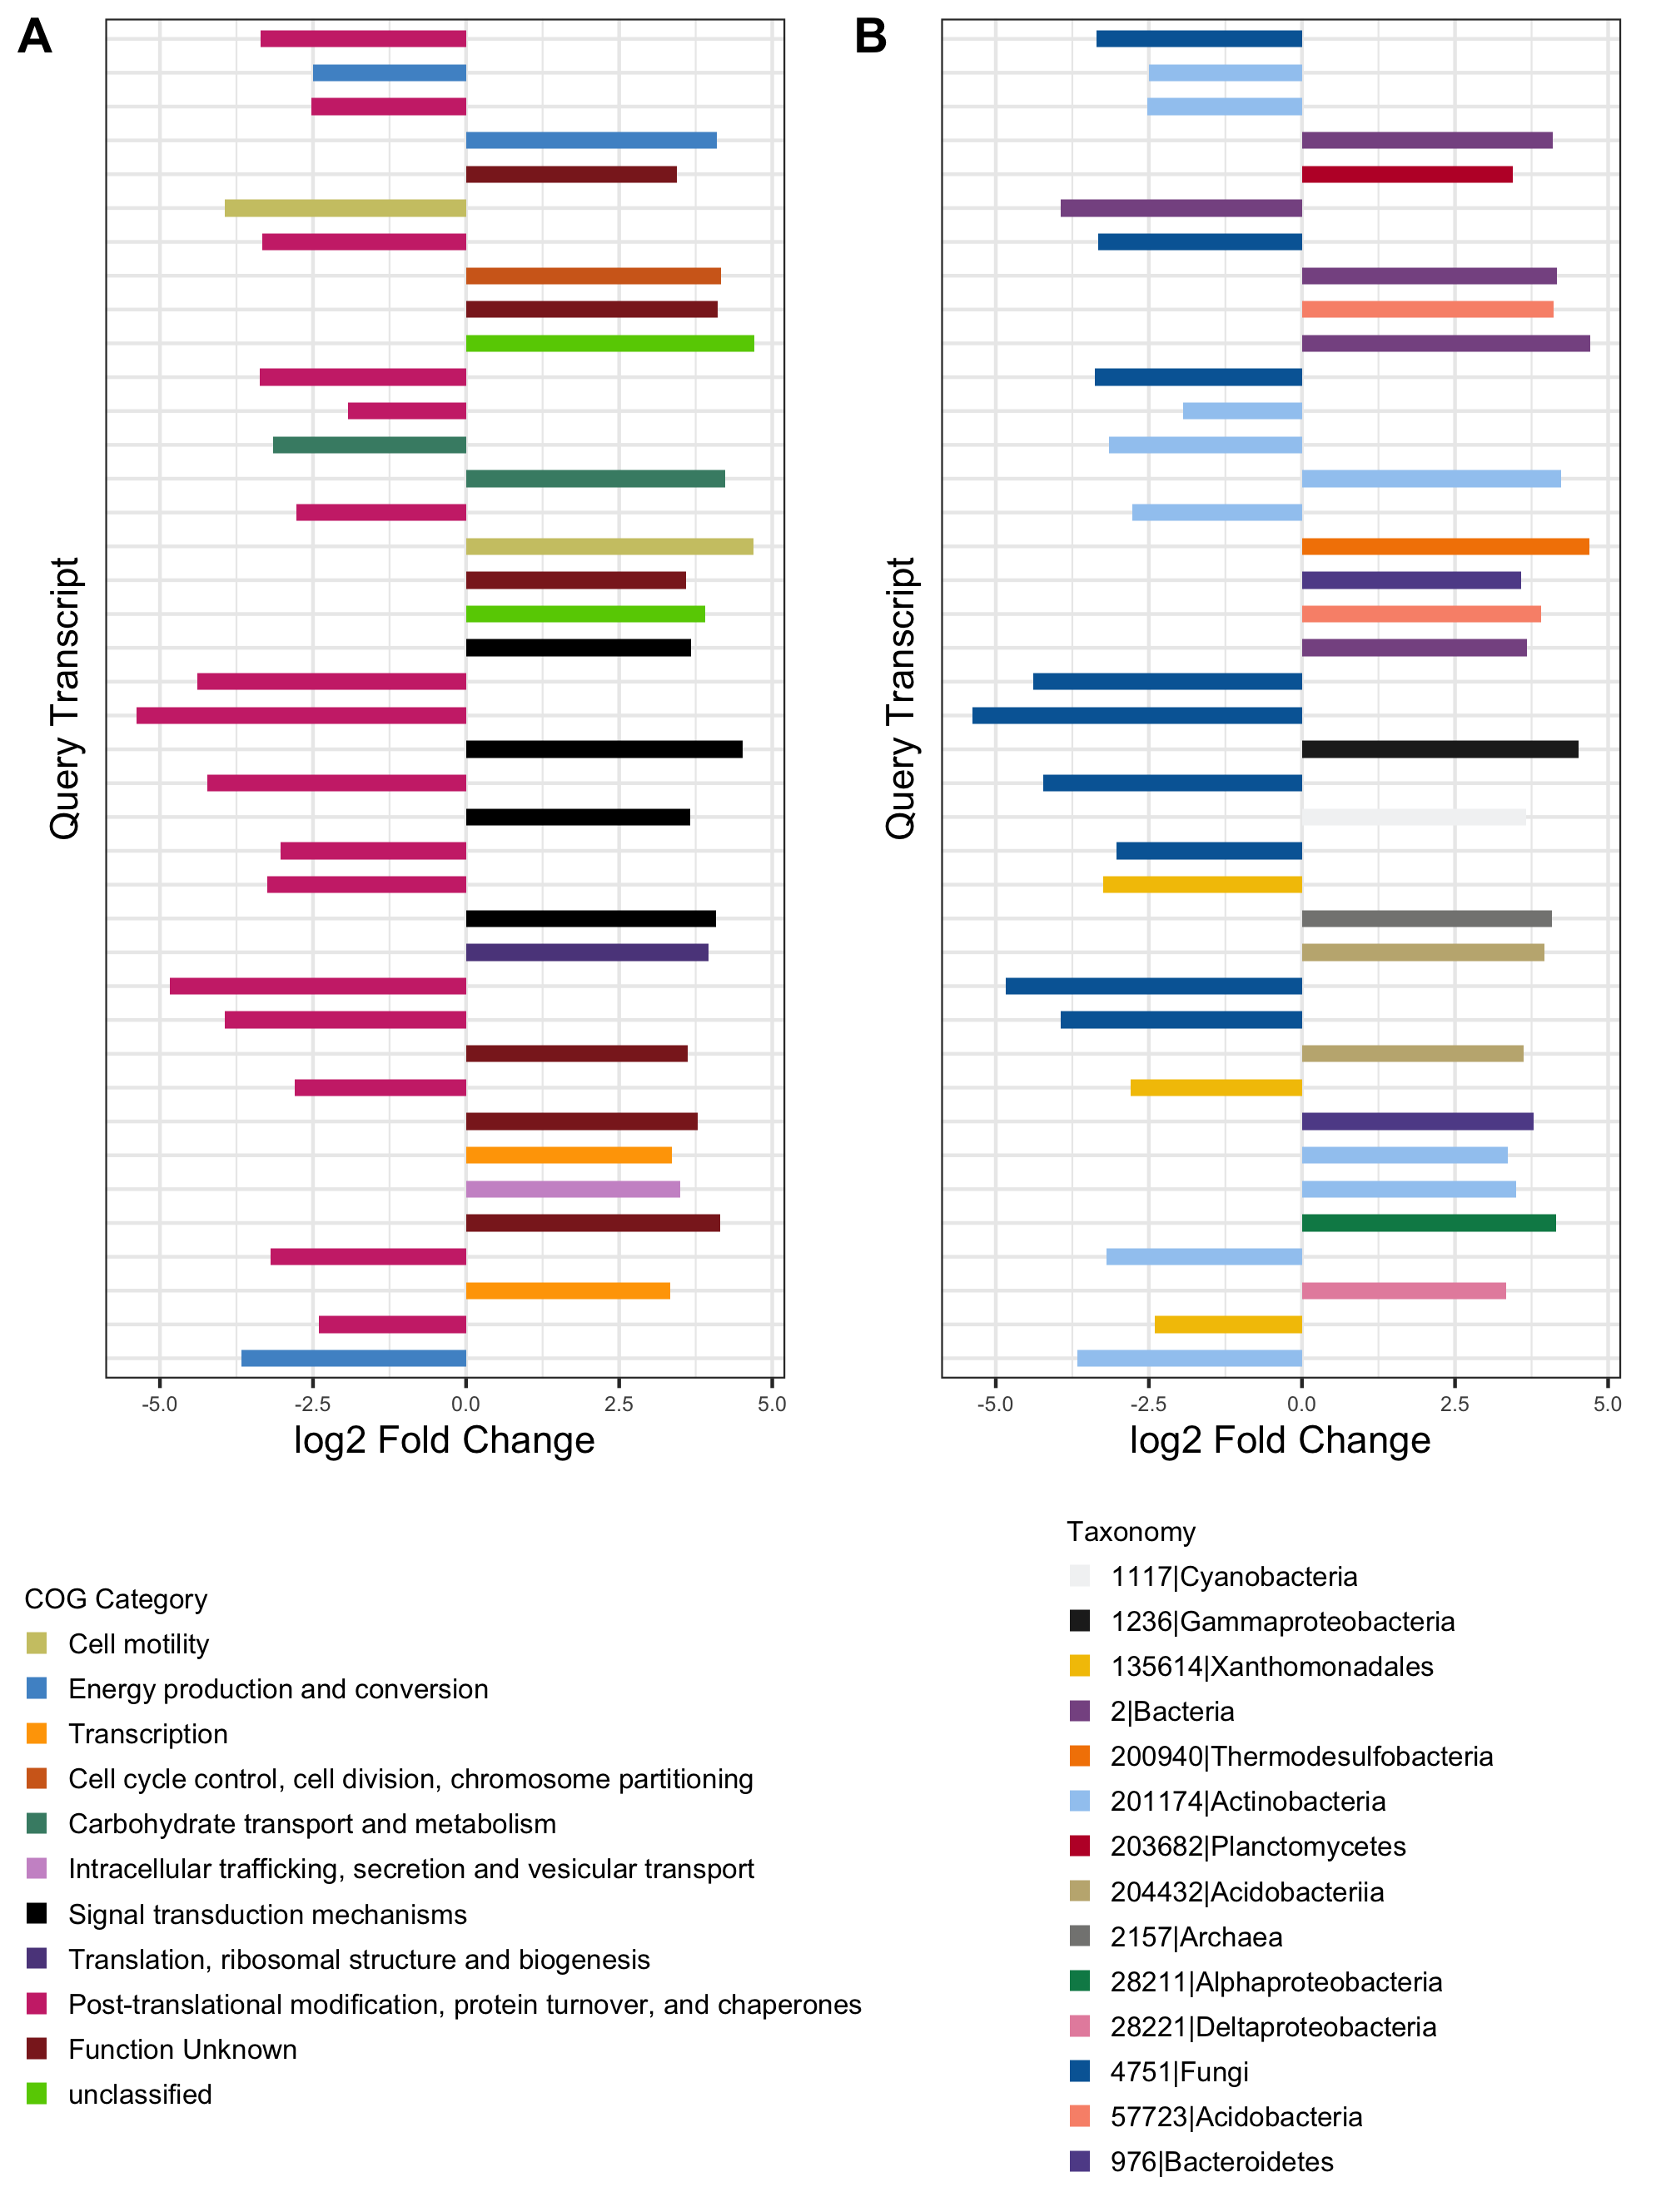
\includegraphics[keepaspectratio]{../../figures/Trt_DE_top20_barplot.png}}

}

\caption{\label{sup-t30-trt-plot}Figure S3. Top 40 up- and
down-regulated genes in controls relative to decomposition soils across
all study days, colored by COG functional category (A) and taxonomic
annotation (B). Positive values denote higher expression in controls,
while negative values are higher in decomposition soils.}

\end{supplemental}%

\begin{supplemental}

\centering{

Table S2. Top 20 most up- and down-regulated gene queries, determined by
log2 fold change and adjusted p-values, in control relative to
decomposition soils. Positive log2 fold change values represent genes
whose expression was higher in control soils, while negative log2 fold
change values were higher in decomposition soils. Taxonomic annotation,
COG categories, gene description, gene names, and EC were assigned via
eggNOG-mapper.

}

\caption{\label{sup-t30-trt-tbl}}

\end{supplemental}%

\begin{supplemental}

\centering{

Table S3. Top 10 most up- and down-regulated genes, determined by log2
fold change and adjusted p-values, for each sequential timepoint
comparison. Positive log2 fold change values represent genes whose
expression was higher in the later decomposition timepoint soils, while
negative log2 fold change values are higher in earlier decomposition
timepoint soils. Taxonomic annotation, COG categories, gene names, and
EC were assigned via eggNOG-mapper. The comparison column distinguishes
each timepoint comparison.

}

\caption{\label{sup-t20-day-tbl}}

\end{supplemental}%

\begin{supplemental}

\centering{

\pandocbounded{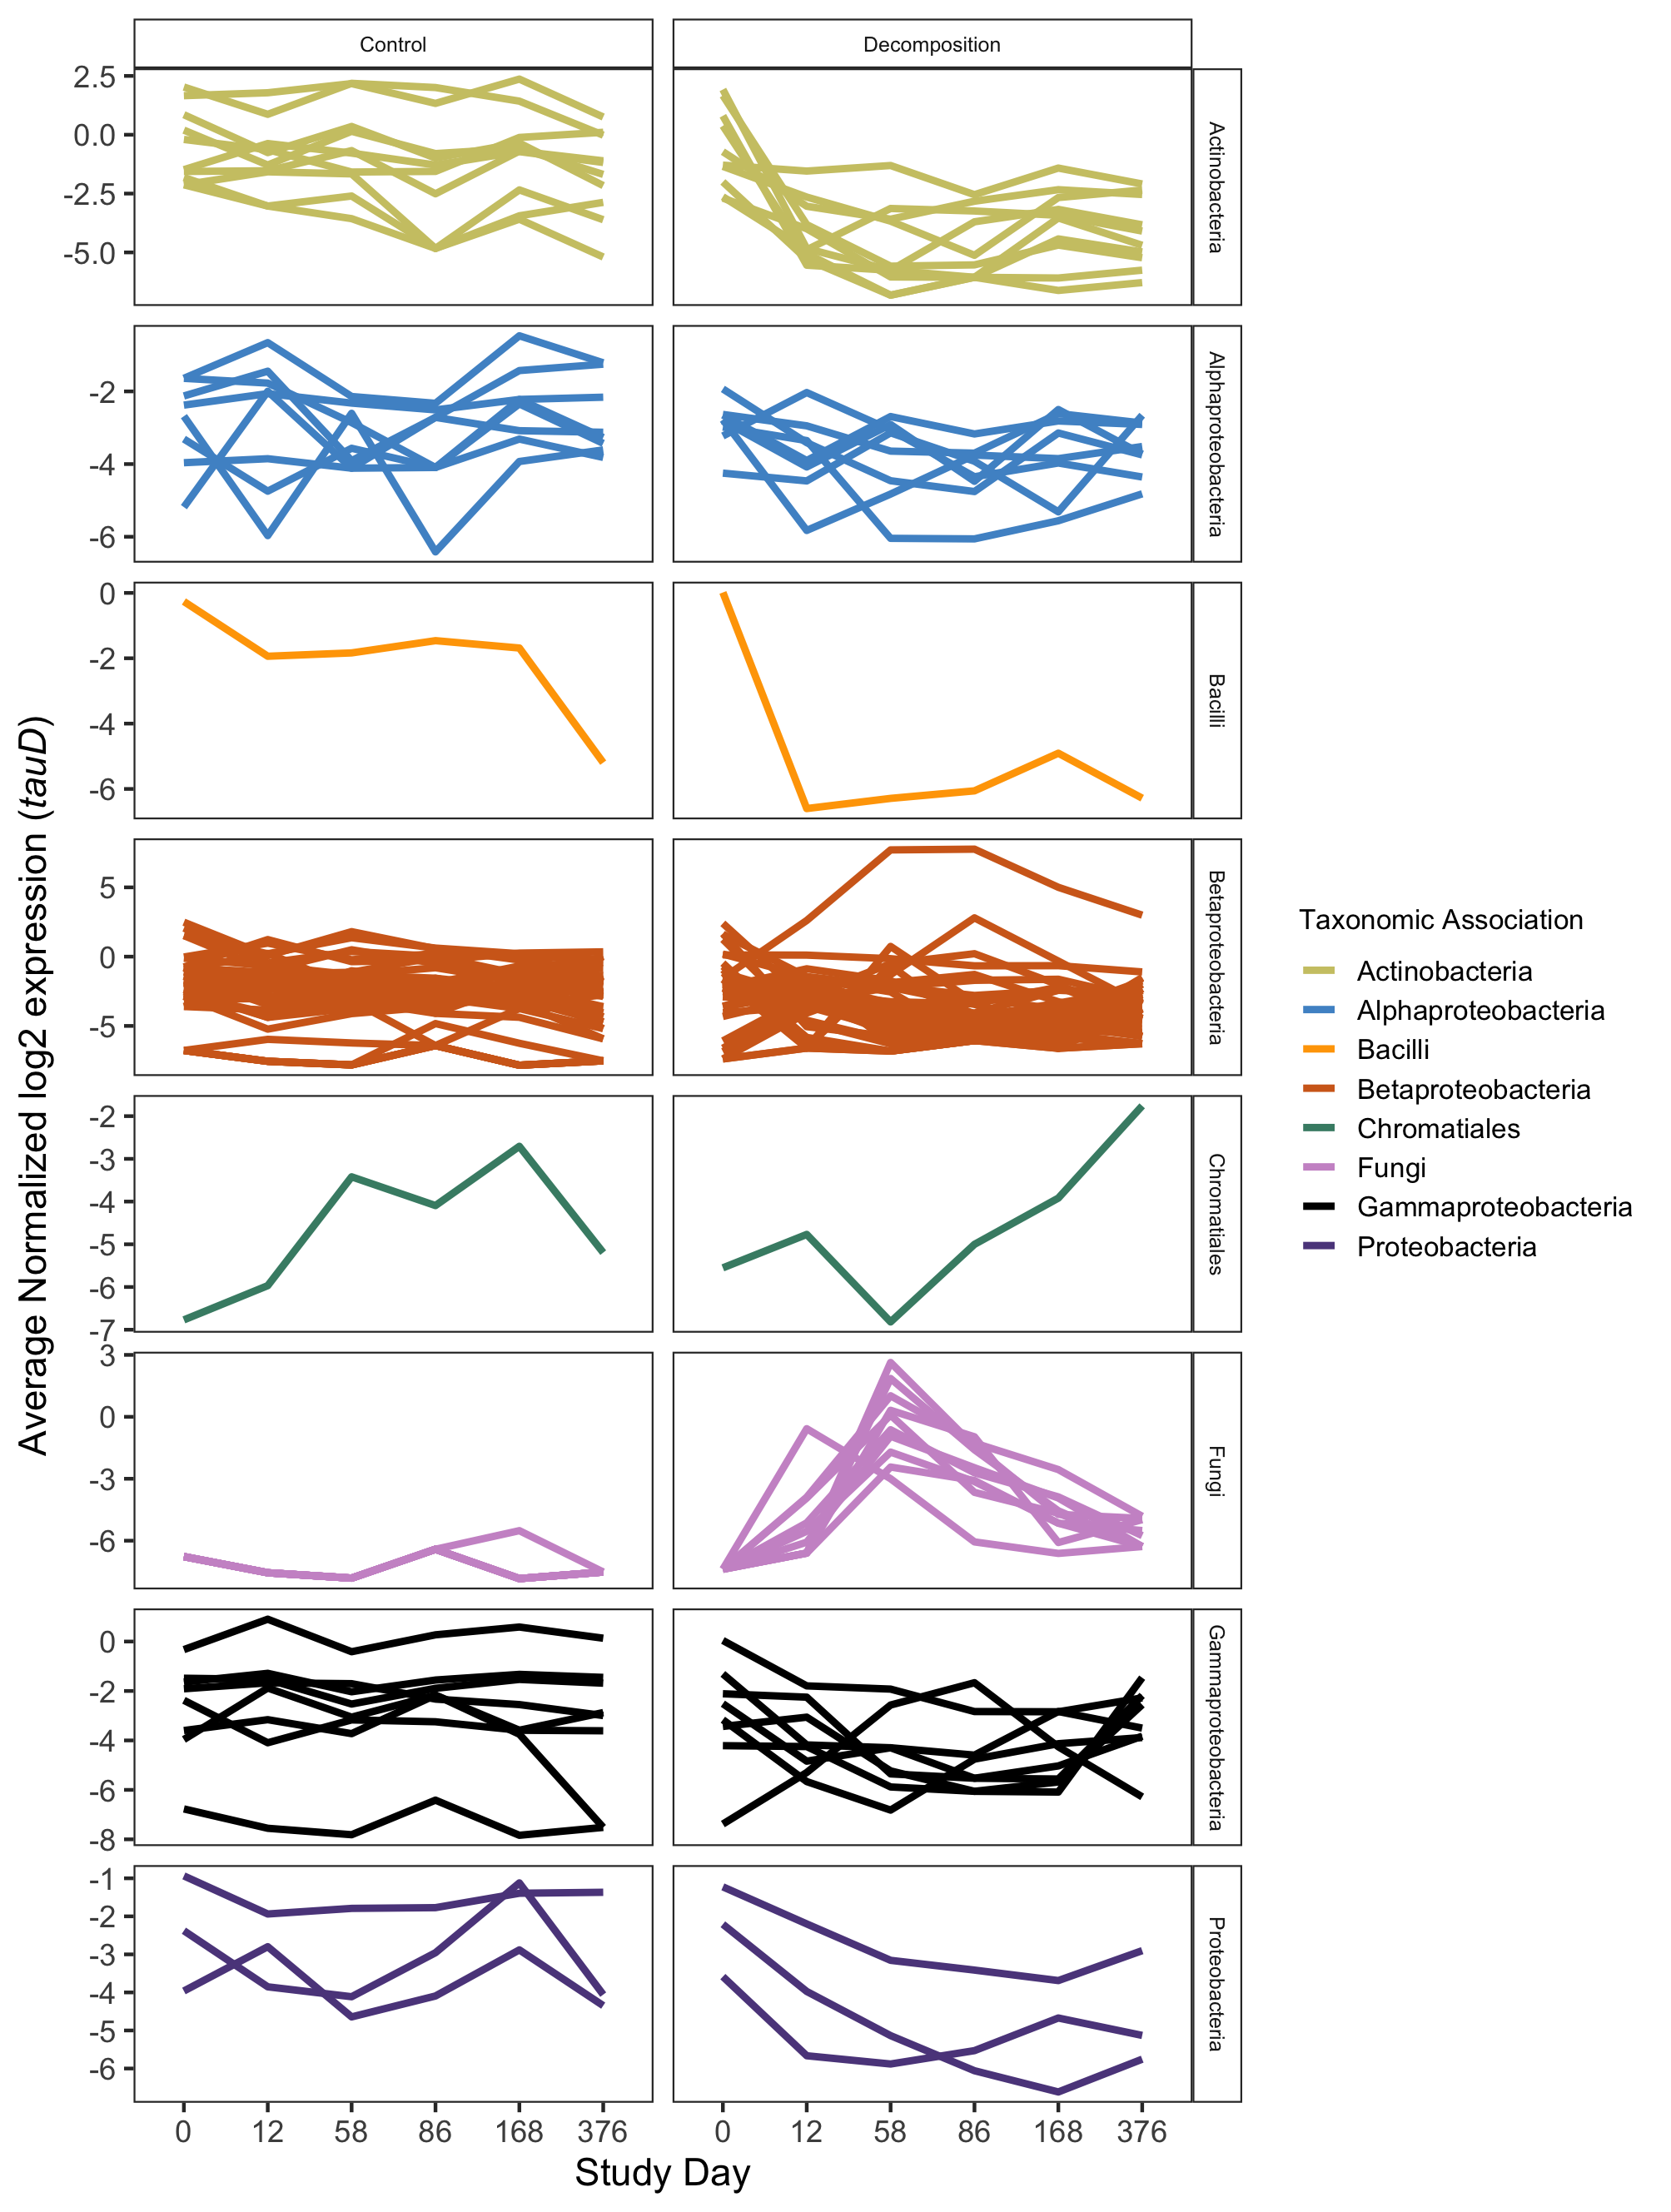
\includegraphics[keepaspectratio]{../../figures/tauD_nlog2_taxonomy.png}}

}

\caption{\label{sup-taud-tax}Figure S4. Mean normalized log2 expression
of \emph{tauD} genes by taxonomic association (color) in control and
decomposition soils at each study day. Each line represents one
\emph{tauD} gene query, while color denotes taxonomic association as
determined by eggNOG-mapper.}

\end{supplemental}%





\end{document}
